% advsync/memorybarriers.tex

\section{Memory Barriers}
\label{sec:advsync:Memory Barriers}
\OriginallyPublished{Section}{sec:advsync:Memory Barriers}{Linux Kernel Memory Barriers}{kernel.org}{Howells2009membartxt}

Causality and sequencing are deeply intuitive, and hackers often
tend to have a much stronger grasp of these concepts than does
the general population.
These intuitions can be extremely powerful tools when writing, analyzing,
and debugging both sequential code and parallel code that makes
use of standard mutual-exclusion mechanisms, such as locking and
RCU.

\begin{listing}
{ \scriptsize
\begin{verbbox}[\LstLineNo]
C C-SB+o-o+o-o
{
}

P0(int *x0, int *x1)
{
  int r2;

  WRITE_ONCE(*x0, 2);
  r2 = READ_ONCE(*x1);
}


P1(int *x0, int *x1)
{
  int r2;

  WRITE_ONCE(*x1, 2);
  r2 = READ_ONCE(*x0);
}

exists (1:r2=0 /\ 0:r2=0)
\end{verbbox}
}
\centering
\theverbbox
\caption{Memory Misordering: Store-Buffering Litmus Test}
\label{lst:advsync:Memory Misordering: Store-Buffering Litmus Test}
\end{listing}

Unfortunately, these intuitions break down completely in face of
code that fails to use standard mechanisms.
For example, the trivial-seeming litmus test in
Listing~\ref{lst:advsync:Memory Misordering: Store-Buffering Litmus Test}
(\path{C-SB+o-o+o-o.litmus})
appears to guarantee that the \co{exists} clause never triggers.\footnote{
	Purists would instead say that the \co{exists} clause is
	never \emph{satisfied}, but we use ``trigger'' here by
	analogy with assertions.}
After all, if \nbco{0:r2=0} as shown in the \co{exists} clause,\footnote{
	That is, Thread~\co{P0()}'s instance of local variable \co{r2}
	equals zero.
	See Section~\ref{sec:formal:Anatomy of a Litmus Test}
	for documentation of litmus-test nomenclature.}
we might hope that Thread~\co{P0()}'s
load from~\co{x1} must have happened before Thread~\co{P1()}'s store to~\co{x1},
which might raise
further hopes that Thread~\co{P1()}'s load from~\co{x0} must happen after
Thread~\co{P0()}'s store to~\co{x0}, so that \nbco{1:r2=2},
thus not triggering the \co{exists} clause.
The example is symmetric, so similar reasoning might lead
us to hope that \nbco{1:r2=0} guarantees that \nbco{0:r2=2}.
Unfortunately, the lack of memory barriers dashes these hopes.
Both the compiler and the CPU are within their rights to reorder
the statements within both Thread~\co{P0()} and Thread~\co{P1()},
even on relatively strongly ordered systems such as x86.

This willingness to reorder can be confirmed using tools such as
\co{litmus7}~\cite{Alglave:2014:HCM:2594291.2594347},
which found that the counter-intuitive ordering happened
314 times out of 100,000,000 trials on my x86 laptop.
Oddly enough, the perfectly legal outcome where both loads return the
value 2 occurred less frequently, in this case, only 167 times.\footnote{
	Please note that results are sensitive to the exact hardware
	configuration,
	how heavily the system is loaded, and much else besides.}
The lesson here is clear: Increased counterintuitivity does not necessarily
imply decreased probability!
% Run on June 23, 2017:
% litmus7 -r 1000 -carch X86 C-SB+o-o+o-o.litmus
% Test C-SB+o-o+o-o Allowed
% Histogram (4 states)
% 314   *>0:r2=0; 1:r2=0;
% 49999625:>0:r2=2; 1:r2=0;
% 49999894:>0:r2=0; 1:r2=2;
% 167   :>0:r2=2; 1:r2=2;

The following sections show exactly where this intuition breaks down,
and then puts forward a mental model of memory barriers that can help
you avoid these pitfalls.

Section~\ref{sec:advsync:Memory Ordering and Memory Barriers}
gives a brief overview of memory ordering and memory barriers.
Once this background is in place, the next step is to get you to admit
that your intuition has a problem.
This painful task is taken up by
Section~\ref{sec:advsync:Variables Can Have More Than One Value},
which presents some code demonstrating that scalar variables can
take on multiple values simultaneously,
and by
Section~\ref{sec:advsync:If B Follows A, and C Follows B, Why Doesn't C Follow A?},
which shows an intuitively correct code fragment that fails miserably
on real hardware.
Once your intuition has made it through the grieving process,
Section~\ref{sec:advsync:What Can You Trust?}
provides the basic rules that memory barriers follow, rules that we
will build upon.
These rules are further refined in
Sections~\ref{sec:advsync:Review of Locking Implementations}
through~\ref{sec:advsync:Where Are Memory Barriers Needed?}.

\subsection{Memory Ordering and Memory Barriers}
\label{sec:advsync:Memory Ordering and Memory Barriers}

But why are memory barriers needed in the first place?
Can't CPUs keep track of ordering on their own?
Isn't that why we have computers in the first place, to keep track of things?

Many people do indeed expect their computers to keep track of things,
but many also insist that they keep track of things quickly.
However, as seen in Chapter~\ref{chp:Hardware and its Habits},
one difficulty that modern computer-system vendors face is that
the main memory cannot keep up with the CPU---modern CPUs can execute
hundreds of instructions in the time required to fetch a single variable
from memory.
CPUs therefore sport increasingly large caches, as seen back in
Figure~\ref{fig:cpu:System Hardware Architecture}, which means that
although the first load by a given CPU from a given variable will
result in an expensive \emph{cache miss} as was discussed in
Section~\ref{sec:cpu:Cache Misses}, subsequent
repeated loads from that variable by that CPU can execute
very quickly because the initial cache miss will have loaded that
variable into that CPU's cache.

However, it is also necessary to accommodate frequent concurrent stores
from multiple CPUs to a set of shared variables.
In cache-coherent systems, if the caches hold multiple copies of a given
variable, all the copies of that variable must have the same value.
This works extremely well for concurrent reads, but not so well for
concurrent writes:  Each write must do something about all
copies of the old value (another cache miss!), which, given the finite
speed of light and the atomic nature of matter, will be slower
than impatient software hackers would like.

\begin{figure}[tb]
\centering
\resizebox{2.5in}{!}{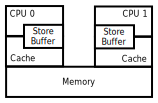
\includegraphics{advsync/SystemArchSB}}
\caption{System Architecture With Store Buffers}
\label{fig:advsync:System Architecture With Store Buffers}
\end{figure}

CPUs therefore come equipped with store buffers, as shown in
Figure~\ref{fig:advsync:System Architecture With Store Buffers}.
When a given CPU does a store to a given variable when that
variable is not present in that CPU's cache, then the new value
is instead placed in that CPU's store buffer.
The CPU can then proceed immediately, without having to wait for the
store to do something about all the old values of that variable
residing in other CPUs' caches.

\begin{figure}[htb]
\centering
\resizebox{3in}{!}{\includegraphics{cartoons/r-2014-Out-of-order}}
\caption{CPUs Can Do Things Out of Order}
\ContributedBy{Figure}{fig:advsync:CPUs Can Do Things Out of Order}{Melissa Broussard}
\end{figure}

Although store buffers can greatly increase performance,
they can cause instructions and memory references to execute out
of order, which can in turn cause serious confusion, as illustrated in
Figure~\ref{fig:advsync:CPUs Can Do Things Out of Order}.
In particular, these store buffers can cause the memory misordering
shown in the store-buffering litmus test in
Listing~\ref{lst:advsync:Memory Misordering: Store-Buffering Litmus Test}.

\begin{table*}
\small
\centering\OneColumnHSpace{-0.1in}
\begin{tabular}{r||l|l|l||l|l|l}
	& \multicolumn{3}{c||}{CPU 0} & \multicolumn{3}{c}{CPU 1} \\
	\cline{2-7}
	& Instruction & Store Buffer & Cache &
		Instruction & Store Buffer & Cache \\
	\hline
	\hline
	1 & (Initial state) & & \tco{x1==0} &
		(Initial state) & & \tco{x0==0} \\
	\hline
	2 & \tco{x0 = 2;} & \tco{x0==2} & \tco{x1==0} &
		\tco{x1 = 2;} & \tco{x1==2} & \tco{x0==0} \\
	\hline
	3 & \tco{r2 = x1;} (0) & \tco{x0==2} & \tco{x1==0} &
		\tco{r2 = x0;} (0) & \tco{x1==2} & \tco{x0==0} \\
	\hline
	4 & (Read-invalidate) & \tco{x0==2} & \tco{x0==0} &
		(Read-invalidate) & \tco{x1==2} & \tco{x1==0} \\
	\hline
	5 & (Finish store) & & \tco{x0==2} &
		(Finish store) & & \tco{x1==2} \\
\end{tabular}
\caption{Memory Misordering: Store-Buffering Sequence of Events}
\label{tab:advsync:Memory Misordering: Store-Buffering Sequence of Events}
\end{table*}

Table~\ref{tab:advsync:Memory Misordering: Store-Buffering Sequence of Events}
shows how this memory misordering can happen.
Row~1 shows the initial state, where CPU~0 has \co{x1} in its cache
and CPU~1 has \co{x0} in its cache, both variables having a value of zero.
Row~2 shows the state change due to each CPU's store (lines~9 and~18 of
Listing~\ref{lst:advsync:Memory Misordering: Store-Buffering Litmus Test}).
Because neither CPU has the stored-to variable in its cache, both CPUs
record their stores in their respective store buffers.

\QuickQuiz{}
	But wait!!!
	On row~2 of
	Table~\ref{tab:advsync:Memory Misordering: Store-Buffering Sequence of Events}
	both \co{x0} and \co{x1} each have two values at the same time,
	namely zero and two.
	How can that possibly work???
\QuickQuizAnswer{
	There is an underlying cache-coherence protocol that straightens
	things out, which will be discussed later.
	% @@@ Add forward reference.
	But if you think that a given variable having two values at
	the same time is surprising, just wait until you get to
	Section~\ref{sec:advsync:Variables Can Have More Than One Value}!
} \QuickQuizEnd

Row~3 shows the two reads (lines~10 and~19 of
Listing~\ref{lst:advsync:Memory Misordering: Store-Buffering Litmus Test}).
Because the variable being read by each CPU is in that CPU's cache,
each read immediately returns the cached value, which in both cases
is zero.

But the CPUs are not done yet: Sooner or later, they must empty their
store buffers.
Because caches move data around in relatively large blocks called
\emph{cachelines}, and because each cacheline can hold several
variables, each CPU must get the cacheline into its own cache so
that it can update the portion of that cacheline corresponding
to the variable in its store buffer, but without disturbing any
other part of the cacheline.
Each CPU must also ensure that the cacheline is not present in any other
CPU's cache, for which a read-invalidate operation is used.
As shown on row~4, after both read-invalidate operations complete,
the two CPUs have traded cachelines, so that CPU~0's cache now contains
\co{x0} and CPU~1's cache now contains \co{x1}.
Once these two variables are in their new homes, each CPU can flush
its store buffer into the corresponding cache line, leaving each
variable with its final value as shown on row~5.

\QuickQuiz{}
	But don't the values also need to be flushed from the cache
	to main memory?
\QuickQuizAnswer{
	Perhaps surprisingly, not necessarily!
	On some systems,
	if the two variables are being used heavily, they might
	be bounced back and forth between the CPUs' caches and never
	land in main memory.
} \QuickQuizEnd

In summary, store buffers are needed to allow CPUs to handle
store instructions efficiently, but they can result in
counter-intuitive memory misordering.

But what do you do if your algorithm really needs its memory
references to be ordered?
It turns out that there are compiler directives and standard
synchronization primitives (such as locking and RCU)
that are responsible for maintaining the illusion of ordering through use of
\emph{memory barriers} (for example, \co{smp_mb()} in the Linux kernel).
These memory barriers can be explicit instructions, as they are on
ARM, POWER, Itanium, and Alpha, or they can be implied by other instructions,
as they often are on x86.
Since these standard synchronization primitives preserve the illusion of
ordering, your path of least resistance is to simply use these primitives,
thus allowing you to stop reading this section.

\begin{listing}
{ \scriptsize
\begin{verbbox}[\LstLineNo]
C C-SB+o-mb-o+o-mb-o
{
}

P0(int *x0, int *x1)
{
  int r2;

  WRITE_ONCE(*x0, 2);
  smp_mb();
  r2 = READ_ONCE(*x1);
}


P1(int *x0, int *x1)
{
  int r2;

  WRITE_ONCE(*x1, 2);
  smp_mb();
  r2 = READ_ONCE(*x0);
}

exists (1:r2=0 /\ 0:r2=0)
\end{verbbox}
}
\centering
\theverbbox
\caption{Memory Ordering: Store-Buffering Litmus Test}
\label{lst:advsync:Memory Ordering: Store-Buffering Litmus Test}
\end{listing}

However, if you need to implement the synchronization primitives
themselves, or if you are simply interested in understanding how memory
ordering and memory barriers work, read on!
The first stop is
Listing~\ref{lst:advsync:Memory Ordering: Store-Buffering Litmus Test}
(\path{C-SB+o-mb-o+o-mb-o.litmux}),
which the \co{smp_mb()} Linux-kernel full memory barrier placed between
the store and load in both \co{P0()} and \co{P1()}, but is otherwise
identical to the code shown in
Listing~\ref{lst:advsync:Memory Misordering: Store-Buffering Litmus Test}.
% Test C-SB+o-mb-o+o-mb-o Allowed
% Histogram (3 states)
% 49553298:>0:r2=2; 1:r2=0;
% 49636449:>0:r2=0; 1:r2=2;
% 810253:>0:r2=2; 1:r2=2;
% No
These directives prevent the counter-intuitive outcome from happening
on 100,000,000 trials on my x86 laptop.
Interestingly enough, the overhead of these directives causes the
legal outcome where both loads return the value two to happen more
than 800,000 times, as opposed to only 167 times for the
directive-free code in
Listing~\ref{lst:advsync:Memory Misordering: Store-Buffering Litmus Test}.

\begin{table*}
\small
\centering\OneColumnHSpace{-0.1in}
\begin{tabular}{r||l|l|l||l|l|l}
	& \multicolumn{3}{c||}{CPU 0} & \multicolumn{3}{c}{CPU 1} \\
	\cline{2-7}
	& Instruction & Store Buffer & Cache &
		Instruction & Store Buffer & Cache \\
	\hline
	\hline
	1 & (Initial state) & & \tco{x1==0} &
		(Initial state) & & \tco{x0==0} \\
	\hline
	2 & \tco{x0 = 2;} & \tco{x0==2} & \tco{x1==0} &
		\tco{x1 = 2;} & \tco{x1==2} & \tco{x0==0} \\
	\hline
	3 & \tco{smp_mb();} & \tco{x0==2} & \tco{x1==0} &
		\tco{smp_mb();} & \tco{x1==2} & \tco{x0==0} \\
	\hline
	4 & (Read-invalidate) & \tco{x0==2} & \tco{x0==0} &
		(Read-invalidate) & \tco{x1==2} & \tco{x1==0} \\
	\hline
	5 & (Finish store) & & \tco{x0==2} &
		(Finish store) & & \tco{x1==2} \\
	\hline
	6 & \tco{r2 = x1;} (2) & & \tco{x1==2} &
		\tco{r2 = x0;} (2) & & \tco{x0==2} \\
\end{tabular}
\caption{Memory Ordering: Store-Buffering Sequence of Events}
\label{tab:advsync:Memory Ordering: Store-Buffering Sequence of Events}
\end{table*}

These directives have a profound effect on ordering, as can be seen in
Table~\ref{tab:advsync:Memory Ordering: Store-Buffering Sequence of Events}.
Although the \co{smp_mb()} instructions on row~3
do not change state
in and of themselves, they do cause the stores to complete before the
loads, which rules out the counter-intuitive outcome shown in
Table~\ref{tab:advsync:Memory Misordering: Store-Buffering Sequence of Events}.
Note that variables \co{x0} and \co{x1} each still have more than one
value on row~2, however, as promised earlier, the directives straighten
things out in the end.

Please note that actual hardware tends to be much more complex, tricky,
and subtle than is described here.
After all, the point of this discussion is not to train you to be
a hardware architect, but rather to help you correctly code
low-level concurrent primitives.
But first, let's take a quick look at just how many values a single
variable might have at a single moment of time.

\subsection{Variables Can Have More Than One Value}
\label{sec:advsync:Variables Can Have More Than One Value}

It is natural to think of a variable as taking on a well-defined
sequence of values in a well-defined, global order.
Unfortunately, it is time to say ``goodbye'' to this comforting fiction.
Hopefully, you already started to say ``goodbye'' in response to row~2 of
Tables~\ref{tab:advsync:Memory Misordering: Store-Buffering Sequence of Events}
and~\ref{tab:advsync:Memory Ordering: Store-Buffering Sequence of Events},
but either way, the purpose of this section is to drive this point home.

To this end, consider the program fragment shown in
Listing~\ref{lst:advsync:Software Logic Analyzer}.
This code fragment is executed in parallel by several CPUs.
Line~1 sets a shared variable to the current CPU's ID, line~2
initializes several variables from a \co{gettb()} function that
delivers the value of a fine-grained hardware ``timebase'' counter that is
synchronized among all CPUs (not available from all CPU architectures,
unfortunately!), and the loop from lines~3-8 records the length of
time that the variable retains the value that this CPU assigned to it.
Of course, one of the CPUs will ``win'', and would thus never exit
the loop if not for the check on lines~6-7.

\QuickQuiz{}
	What assumption is the code fragment
	in Listing~\ref{lst:advsync:Software Logic Analyzer}
	making that might not be valid on real hardware?
\QuickQuizAnswer{
	The code assumes that as soon as a given CPU stops
	seeing its own value, it will immediately see the
	final agreed-upon value.
	On real hardware, some of the CPUs might well see several
	intermediate results before converging on the final value.
} \QuickQuizEnd

\begin{listing}[tbp]
{ \scriptsize
\begin{verbbox}
  1 state.variable = mycpu;
  2 lasttb = oldtb = firsttb = gettb();
  3 while (state.variable == mycpu) {
  4   lasttb = oldtb;
  5   oldtb = gettb();
  6   if (lasttb - firsttb > 1000)
  7     break;
  8 }
\end{verbbox}
}
\centering
\theverbbox
\caption{Software Logic Analyzer}
\label{lst:advsync:Software Logic Analyzer}
\end{listing}

Upon exit from the loop, \co{firsttb} will hold a timestamp
taken shortly after the assignment and \co{lasttb} will hold
a timestamp taken before the last sampling of the shared variable
that still retained the assigned value, or a value equal to \co{firsttb}
if the shared variable had changed before entry into the loop.
This allows us to plot each CPU's view of the value of \co{state.variable}
over a 532-nanosecond time period, as shown in
Figure~\ref{fig:advsync:A Variable With Multiple Simultaneous Values}.
This data was collected in 2006 on 1.5\,GHz POWER5 system with 8 cores,
each containing a pair of hardware threads.
CPUs~1, 2, 3, and~4 recorded the values, while CPU~0 controlled the test.
The timebase counter period was about 5.32\,ns, sufficiently fine-grained
to allow observations of intermediate cache states.

\begin{figure}[htb]
\centering
\resizebox{3in}{!}{\includegraphics{advsync/MoreThanOneValue}}
\caption{A Variable With Multiple Simultaneous Values}
\label{fig:advsync:A Variable With Multiple Simultaneous Values}
\end{figure}

Each horizontal bar represents the observations of a given CPU over time,
with the black regions to the left indicating the time before the
corresponding CPU's first measurement.
During the first 5\,ns, only CPU~3 has an opinion about the value of the
variable.
During the next 10\,ns, CPUs~2 and~3 disagree on the value of the variable,
but thereafter agree that the value is~``2'', which is in fact
the final agreed-upon value.
However, CPU~1 believes that the value is~``1'' for almost 300\,ns, and
CPU~4 believes that the value is~``4'' for almost 500\,ns.

\QuickQuiz{}
	How could CPUs possibly have different views of the
	value of a single variable \emph{at the same time?}
\QuickQuizAnswer{
	Many CPUs have write buffers that record the values of
	recent writes, which are applied once the corresponding
	cache line makes its way to the CPU.
	Therefore, it is quite possible for each CPU to see a
	different value for a given variable at a single point
	in time---and for main memory to hold yet another value.
	One of the reasons that memory barriers were invented was
	to allow software to deal gracefully with situations like
	this one.
} \QuickQuizEnd

\QuickQuiz{}
	Why do CPUs~2 and~3 come to agreement so quickly, when it
	takes so long for CPUs~1 and~4 to come to the party?
\QuickQuizAnswer{
	CPUs~2 and~3 are a pair of hardware threads on the same
	core, sharing the same cache hierarchy, and therefore have
	very low communications latencies.
	This is a NUMA, or, more accurately, a NUCA effect.

	This leads to the question of why CPUs~2 and~3 ever disagree
	at all.
	One possible reason is that they each might have a small amount
	of private cache in addition to a larger shared cache.
	Another possible reason is instruction reordering, given the
	short 10-nanosecond duration of the disagreement and the
	total lack of memory barriers in the code fragment.
} \QuickQuizEnd

And if you think that the situation with four CPUs was intriguing, consider
Figure~\ref{fig:advsync:A Variable With More Simultaneous Values},
which shows the same situation, but with 15~CPUs each assigning their
number to a single shared variable at time~$t=0$. Both diagrams in the
figure are drawn in the same way as 
Figure~\ref{fig:advsync:A Variable With Multiple Simultaneous Values}.
The only difference is that the unit of horizontal axis is timebase ticks,
with each tick lasting about 5.3~nanoseconds.
The entire sequence therefore lasts a bit longer than the events recorded in
Figure~\ref{fig:advsync:A Variable With Multiple Simultaneous Values},
consistent with the increase in number of CPUs.
The upper diagram shows the overall picture, while the lower one shows
the zoom-up of first 50~timebase ticks.

Again, CPU~0 coordinates the test, so does not record any values.

\begin{figure*}
\centering
\resizebox{5in}{!}{\includegraphics{advsync/MoreThanOneValue-15CPU}}
\caption{A Variable With More Simultaneous Values}
\ContributedBy{Figure}{fig:advsync:A Variable With More Simultaneous Values}{Akira Yokosawa}
\end{figure*}

All CPUs eventually agree on the final value of~9, but not before
the values~15 and~12 take early leads.
Note that there are fourteen different opinions on the variable's value
at time~21 indicated by the vertical line in the lower diagram.
Note also that all CPUs see sequences whose orderings are consistent with
the directed graph shown in
Figure~\ref{fig:advsync:Possible Global Orders With More Simultaneous Values}.
Nevertheless, both figures underscore the importance of
proper use of memory barriers for code that cares about memory ordering.

\begin{figure}[htb]
\centering
\resizebox{2.5in}{!}{\includegraphics{advsync/store15tred}}
\caption{Possible Global Orders With More Simultaneous Values}
\label{fig:advsync:Possible Global Orders With More Simultaneous Values}
\end{figure}

How many values can a single variable take on at a single point in
time?
As many as one per store buffer in the system!
We have therefore entered a regime where we must bid a fond farewell to
comfortable intuitions about values of variables and the passage of time.
This is the regime where memory barriers are needed.

All that aside, it is important to remember the lessons from
Chapters~\ref{chp:Hardware and its Habits}
and~\ref{cha:Partitioning and Synchronization Design}.
Having all CPUs write concurrently to the same variable
is absolutely no way to design a parallel program, at least
not if performance and scalability are at all important to you.

Unfortunately, memory ordering has many other ways of insulting your
intuition, and not all of these ways conflict with performance and
scalability.
The next section will give an overview of a few of these insults.

\subsection{If B Follows A, and C Follows B, Why Doesn't C Follow A?}
\label{sec:advsync:If B Follows A, and C Follows B, Why Doesn't C Follow A?}

Why indeed?
This section will help to answer this question, in part by looking
more closely at what ``follows'' might mean.

\subsubsection{Memory-Reference Reordering}
\label{sec:advsync:Memory-Reference Reordering}

Section~\ref{sec:advsync:Memory Ordering and Memory Barriers}
showed that even relatively strongly ordered systems like x86
can reorder prior stores with later loads, at least when the
store and load are to different variables.
This section buids on that result, looking at the other combinations of
loads and stores.

% @@@ Rationale for further reordering.

\begin{listing}[tbp]
{ \scriptsize
\begin{verbbox}[\LstLineNo]
C C-MP+o-wmb-o+o-o.litmus

{
}


P0(int* x0, int* x1) {

  WRITE_ONCE(*x0, 2);
  smp_wmb();
  WRITE_ONCE(*x1, 2);

}

P1(int* x0, int* x1) {

  int r2;
  int r3;

  r2 = READ_ONCE(*x1);
  r3 = READ_ONCE(*x0);

}

exists (1:r2=2 /\ 1:r3=0)
\end{verbbox}
}
\centering
\theverbbox
\caption{Message-Passing Litmus Test}
\label{lst:advsync:Message-Passing Litmus Test}
\end{listing}

\paragraph{Load Followed By Load:}
Listing~\ref{lst:advsync:Message-Passing Litmus Test}
shows the classic \emph{message-passing} litmus test, where \co{x0} is
the message and \co{x1} is a flag indicating whether or not a message
is available.
In this test, the \co{smp_wmb()} forces \co{P0()} writes to be ordered,
but there is no ordering specified for the reads.
Relatively strongly ordered architectures, such as x86, do enforce ordering.
However, weakly ordered archictures do not necessarily enforce
this~\cite{JadeAlglave2011ppcmem}.
Therefore, the \co{exists} clause on line~25 of the figure \emph{can}
trigger.

\begin{listing}[tbp]
{ \scriptsize
\begin{verbbox}[\LstLineNo]
C C-MP+o-wmb-o+o-rmb-o.litmus

{
}

P0(int* x0, int* x1) {

  WRITE_ONCE(*x0, 2);
  smp_wmb();
  WRITE_ONCE(*x1, 2);

}

P1(int* x0, int* x1) {

  int r2;
  int r3;

  r2 = READ_ONCE(*x1);
  smp_rmb();
  r3 = READ_ONCE(*x0);

}

exists (1:r2=2 /\ 1:r3=0)
\end{verbbox}
}
\centering
\theverbbox
\caption{Enforcing Order of Message-Passing Litmus Test}
\label{lst:advsync:Enforcing Order of Message-Passing Litmus Test}
\end{listing}

Therefore, portable code relying on ordering in this case should
add explicit ordering, for example, the \co{smp_rmb()} shown on
line~20 of
Listing~\ref{lst:advsync:Enforcing Order of Message-Passing Litmus Test}.
Here, the \co{exists} clause cannot trigger.

\begin{listing}[tbp]
{ \scriptsize
\begin{verbbox}[\LstLineNo]
C C-LB+o-o+o-o
{
}

P0(int *x0, int *x1)
{
  int r2;

  r2 = READ_ONCE(*x1);
  WRITE_ONCE(*x0, 2);
}


P1(int *x0, int *x1)
{
  int r2;

  r2 = READ_ONCE(*x0);
  WRITE_ONCE(*x1, 2);
}

exists (1:r2=2 /\ 0:r2=2)
\end{verbbox}
}
\centering
\theverbbox
\caption{Load-Buffering Litmus Test}
\label{lst:advsync:Load-Buffering Litmus Test}
\end{listing}

\paragraph{Load Followed By Store:}
Listing~\ref{lst:advsync:Load-Buffering Litmus Test}
shows the classic \emph{load-buffering} litmus test.
Although relatively strongly ordered systems such as x86
or the IBM Mainframe do not reorder prior loads with subsequent stores,
more weakly ordered architectures really do allow such
reordering~\cite{JadeAlglave2011ppcmem}.
Therefore, the \co{exists} clause on line~22 really can trigger.

\begin{listing}[tbp]
{ \scriptsize
\begin{verbbox}[\LstLineNo]
C C-LB+o-r+a-o.litmus
{
}

P0(int *x0, int *x1)
{
  int r2;

  r2 = READ_ONCE(*x1);
  smp_store_release(x0, 2);
}


P1(int *x0, int *x1)
{
  int r2;

  r2 = smp_load_acquire(x0);
  WRITE_ONCE(*x1, 2);
}

exists (1:r2=2 /\ 0:r2=2)
\end{verbbox}
}
\centering
\theverbbox
\caption{Enforcing Ordering of Load-Buffering Litmus Test}
\label{lst:advsync:Enforcing Ordering of Load-Buffering Litmus Test}
\end{listing}

Interestingly enough, it is relatively rare for actual hardware to
exhibit this reordering~\cite{LucMaranget2017aarch64}.
Nevertheless, you should enforce any required ordering, for example,
as shown in
Listing~\ref{lst:advsync:Enforcing Ordering of Load-Buffering Litmus Test},
thus preventing the \co{exists} clause on line~22 from triggering.

\begin{listing}[tbp]
{ \scriptsize
\begin{verbbox}[\LstLineNo]
C C-MP+o-o+o-rmb-o.litmus

{
}

P0(int* x0, int* x1) {

  WRITE_ONCE(*x0, 2);
  WRITE_ONCE(*x1, 2);

}

P1(int* x0, int* x1) {

  int r2;
  int r3;

  r2 = READ_ONCE(*x1);
  smp_rmb();
  r3 = READ_ONCE(*x0);

}

exists (1:r2=2 /\ 1:r3=0)
\end{verbbox}
}
\centering
\theverbbox
\caption{Message-Passing Litmus Test, No Writer Ordering}
\label{lst:advsync:Message-Passing Litmus Test, No Writer Ordering}
\end{listing}

\paragraph{Store Followed By Store:}
Listing~\ref{lst:advsync:Message-Passing Litmus Test, No Writer Ordering}
once again shows the classic message-passing litmus test, but without
explicit ordering for \co{P0()}'s writes and with the \co{smp_mb()}
providing ordering for \co{P1()}'s reads.
Again, the relatively strongly ordered architectures do enforce ordering,
but weakly ordered architectures do not necessarily do
so~\cite{JadeAlglave2011ppcmem}, which means that the
\co{exists} clause can trigger..
Therefore, portable code should explicitly order the writes, for
example, as shown in
Listing~\ref{lst:advsync:Enforcing Order of Message-Passing Litmus Test},
thus preventing the \co{exists} clause from triggering.

\subsubsection{Address Dependencies}
\label{sec:advsync:Address Dependencies}

An \emph{address dependency} occurs when the value returned by a load
instruction is used to compute the address used by a later memory-reference
instruction.

\begin{listing}[tbp]
{ \scriptsize
\begin{verbbox}[\LstLineNo]
C C-MP+o-wmb-o+o-ad-o.litmus

{
int y=1;
int *x1 = &y;
}

P0(int* x0, int** x1) {

  WRITE_ONCE(*x0, 2);
  smp_wmb();
  WRITE_ONCE(*x1, x0);

}

P1(int** x1) {

  int *r2;
  int r3;

  r2 = READ_ONCE(*x1);
  r3 = READ_ONCE(*r2);

}

exists (1:r2=x0 /\ 1:r3=1)
\end{verbbox}
}
\centering
\theverbbox
\caption{Message-Passing Address-Dependency Litmus Test}
\label{lst:advsync:Message-Passing Address-Dependency Litmus Test}
\end{listing}

Listing~\ref{lst:advsync:Message-Passing Address-Dependency Litmus Test}
shows a linked variant of the message-passing pattern.
The head pointer is \co{x1}, which initially
references the \co{int} variable \co{y} (line~5), which is in turn 
initialized to the value $1$ (line~4).

\co{P0()} updates head pointer \co{x1} to reference \co{x0} (line~12),
but only afer initializing it to $2$ (line~10) and forcing ordering
(line~11).
\co{P1()} picks up the head pointer \co{x1} (line~21), and then loads
the referenced value (line~22).
There is thus an address dependency from the load on line~21 to the
load on line~22.
In this case, the value return by the load on line~21 is exactly the address
used by the load on line~22, but many variations are possible,
including field access using the C-language \co{->} operator,
addition, subtraction, and array indexing.

One might hope that line~21's load from the head pointer would be ordered
before line~22's dereference.
However, this is not the case on DEC Alpha, which can in effect use
a speculated value for the dependent read, as described in more detail in
Section~\ref{sec:app:whymb:Alpha}.
Therefore,
Listing~\ref{lst:advsync:Message-Passing Address-Dependency Litmus Test}'s
\co{exists} clause \emph{can} trigger.

\begin{listing}[tbp]
{ \scriptsize
\begin{verbbox}[\LstLineNo]
C C-MP+o-wmb-o+ld-ad-o.litmus

{
int y=1;
int *x1 = &y;
}

P0(int* x0, int** x1) {

  WRITE_ONCE(*x0, 2);
  smp_wmb();
  WRITE_ONCE(*x1, x0);

}

P1(int** x1) {

  int *r2;
  int r3;

  r2 = lockless_dereference(*x1);
  r3 = READ_ONCE(*r2);

}

exists (1:r2=x0 /\ 1:r3=1)
\end{verbbox}
}
\centering
\theverbbox
\caption{Enforced Ordering of Message-Passing Address-Dependency Litmus Test}
\label{lst:advsync:Enforced Ordering of Message-Passing Address-Dependency Litmus Test}
\end{listing}

Listing~\ref{lst:advsync:Enforced Ordering of Message-Passing Address-Dependency Litmus Test}
shows how to make this work portably, even on DEC Alpha, by
replacing line~21's \co{READ_ONCE()} with \co{lockless_dereference()},
which acts like \co{READ_ONCE()} on all platforms other than DEC Alpha,
where it acts like a \co{READ_ONCE()} followed by an \co{smp_mb()},
thereby forcing the required ordering on all platforms, and thus
preventing the \co{exists} clause from triggering.

\begin{listing}[tbp]
{ \scriptsize
\begin{verbbox}[\LstLineNo]
C C-S+o-wmb-o+o-ad-o.litmus

{
int y=1;
int *x1 = &y;
}

P0(int* x0, int** x1) {

  WRITE_ONCE(*x0, 2);
  smp_wmb();
  WRITE_ONCE(*x1, x0);

}

P1(int** x1) {

  int *r2;

  r2 = READ_ONCE(*x1);
  WRITE_ONCE(*r2, 3);

}

exists (1:r2=x0 /\ x0=2)
\end{verbbox}
}
\centering
\theverbbox
\caption{S Address-Dependency Litmus Test}
\label{lst:advsync:S Address-Dependency Litmus Test}
\end{listing}

But what happens if the dependent operation is a write rather than
a read, for example, in the \emph{S}
litmus test~\cite{JadeAlglave2011ppcmem} shown in
Listing~\ref{lst:advsync:S Address-Dependency Litmus Test}?
Because no production-quality platform speculates writes,
it is not possible for the \co{WRITE_ONCE()} on line~10 to overwrite
the \co{WRITE_ONCE()} on line~21, meaning that the \co{exists}
clause on line~25 cannot trigger, even on DEC Alpha, even
without the \co{lockless_dereference()} that is required in the
dependent-read case.

\QuickQuiz{}
	But how do we know that \emph{all} platforms really avoid
	triggering the \co{exists} clauses in
	Listings~\ref{lst:advsync:Enforced Ordering of Message-Passing Address-Dependency Litmus Test}
	and~\ref{lst:advsync:S Address-Dependency Litmus Test}?
\QuickQuizAnswer{
	Answering this requires identifying three major groups of platforms:
	(1)~Total-store-order (TSO) platforms,
	(2)~Weakly ordered platorms, and
	(3)~DEC Alpha.

	The TSO platforms order all pairs of memory references except for
	prior stores against later loads.
	Because the address dependency on lines~21 and ~22 of
	Listing~\ref{lst:advsync:Enforced Ordering of Message-Passing Address-Dependency Litmus Test}
	is instead a load followed by another load, TSO platforms preserve
	this address dependency.
	They also preserve the address dependency on lines~20 and~21 of
	Listing~\ref{lst:advsync:S Address-Dependency Litmus Test}
	because this is a load followed by a store, so TSO platforms preserve
	this address dependency as well.
	Because address dependencies must start with a load, TSO platforms
	implicitly but completely respect address dependencies.

	Weakly ordered platforms don't necessarily maintain ordering of
	unrelated accesses.
	However, the address dependencies in
	Listings~\ref{lst:advsync:Enforced Ordering of Message-Passing Address-Dependency Litmus Test}
	and~\ref{lst:advsync:S Address-Dependency Litmus Test}
	are not unrelated: They are related by an address dependency.
	The hardware tracks these dependencies and maintains the needed
	ordering.

	There is one (famous) exception to this rule for weakly ordered
	platforms, and that exception is DEC Alpha for read-to-read
	address dependencies.
	And this is why DEC Alpha requires the explicit memory barrier
	supplied for it by the \co{lockless_dereferenc()} on line~21 of
	Listings~\ref{lst:advsync:Enforced Ordering of Message-Passing Address-Dependency Litmus Test}.
	However, DEC Alpha does track read-to-write address dependendencies,
	which is why line~20 of
	Listings~\ref{lst:advsync:S Address-Dependency Litmus Test}
	does not have a \co{lockless_dereference()}.

	To sum up, current platforms either respect address dependencies
	implicitly, as is the case for TSO platforms (x86, mainframe,
	SPARC, ...), have hardware tracking for address dependencies
	(ARM, PowerPC, MIPS, ...), or have the required memory barriers
	supplied by \co{lockless_dereference()} (DEC Alpha).
} \QuickQuizEnd

However, it is important to note that address dependencies can
be fragile and easily broken by compiler optimizations, as discussed in
Section~\ref{sec:advsync:Address- and Data-Dependency Restrictions}.

\subsubsection{Data Dependencies}
\label{sec:advsync:Data Reordering}

A \emph{data dependency} occurs when the value returned by a load
instruction is used to compute the data stored by a later store
instruction.
Note well the ``data'' above: If the value returned by a load
was instead used to compute the address used by a later store
instruction, that would instead be an address dependency.

\begin{listing}[tbp]
{ \scriptsize
\begin{verbbox}[\LstLineNo]
C C-LB+o-r+o-data-o.litmus
{
}

P0(int *x0, int *x1)
{
  int r2;

  r2 = READ_ONCE(*x1);
  smp_store_release(x0, 2);
}


P1(int *x0, int *x1)
{
  int r2;

  r2 = READ_ONCE(*x0);
  WRITE_ONCE(*x1, r2);
}

exists (1:r2=2 /\ 0:r2=2)
\end{verbbox}
}
\centering
\theverbbox
\caption{Load-Buffering Data-Dependency Litmus Test}
\label{lst:advsync:Load-Buffering Data-Dependency Litmus Test}
\end{listing}

Listing~\ref{lst:advsync:Load-Buffering Data-Dependency Litmus Test}
is similar to
Listing~\ref{lst:advsync:Enforcing Ordering of Load-Buffering Litmus Test},
except that \co{P1()}'s ordering between lines~18 and~19 is
enforced not by an acquire load, but instead by a data dependency:
The value loaded by line~18 is what line~19 stores.
The ordering provided by this data dependency is sufficient to prevent
the \co{exists} clause from triggering.

\QuickQuiz{}
	Why doesn't line~18 of
	Listing~\ref{lst:advsync:Load-Buffering Data-Dependency Litmus Test}
	need a \co{lockless_dereference()}?
\QuickQuizAnswer{
	Data dependencies are always load-to-store dependencies, and
	so all platforms respect them, even DEC Alpha, and for the
	same reasons that they respect load-to-store address dependencies.
} \QuickQuizEnd

Just as with address dependencies, it is important to note that
data dependencies can
be fragile and easily broken by compiler optimizations, as discussed in
Section~\ref{sec:advsync:Address- and Data-Dependency Restrictions}.
In fact, data dependencies can be even more fragile than are address
dependencies.
The reason for this is that address dependencies normally involve
pointer values.
In contrast, as shown in
Listing~\ref{lst:advsync:Load-Buffering Data-Dependency Litmus Test},
it is tempting to carry data dependencies through integral values,
which the compiler has much more freedom to optimize into nonexistence.
For but one example, if the integer loaded was multiplied by the constant
zero, the compiler would know that the result was zero, and could therefore
substitute the constant zero for the value loaded, thus breaking
the dependency.

\QuickQuiz{}
	But wait!!!
	Line~18 of
	Listing~\ref{lst:advsync:Load-Buffering Data-Dependency Litmus Test}
	uses \co{READ_ONCE()}, which marks the load as volatile,
	which means that the compiler absolutely must emit the load
	instruction even if the value is later multiplied by zero.
	So do you really need to work so hard to keep the compiler from
	breaking your data dependancies?
\QuickQuizAnswer{
	Yes, the compiler absolutely must emit a load instruction for
	a volatile load.
	But if you multiply the value loaded by zero, the compiler is
	well within its rights to substitute a constant zero for the
	result of that multiplication, which will break the data
	dependency on many platforms.
} \QuickQuizEnd

In short, you can rely on data dependencies, but only if you take care
to prevent your compiler from breaking them.

\subsubsection{Control Dependencies}
\label{sec:advsync:Control Dependencies}

A \emph{control dependency} occurs when the value returned by a load
instruction is tested to determine whether or not a later store instruction
is executed.
Note well the ``later store instruction'': Many platforms do not respect
load-to-load control dependencies.

\begin{listing}[tbp]
{ \scriptsize
\begin{verbbox}[\LstLineNo]
C C-LB+o-r+o-ctrl-o
{
}

P0(int *x0, int *x1)
{
  int r2;

  r2 = READ_ONCE(*x1);
  smp_store_release(x0, 2);
}


P1(int *x0, int *x1)
{
  int r2;

  r2 = READ_ONCE(*x0);
  if (r2 >= 0)
    WRITE_ONCE(*x1, 2);
}

exists (1:r2=2 /\ 0:r2=2)
\end{verbbox}
}
\centering
\theverbbox
\caption{Load-Buffering Control-Dependency Litmus Test}
\label{lst:advsync:Load-Buffering Control-Dependency Litmus Test}
\end{listing}

Listing~\ref{lst:advsync:Load-Buffering Control-Dependency Litmus Test}
shows another load-buffering example, this time using a control
dependency (line~19) to order the load on line~18 and the store on
line~20.
The ordering is sufficient to prevent the \co{exists} from triggering.

However, control dependencies are even more susceptible to being optimized
out of existence than are data dependencies, and
Section~\ref{sec:advsync:Control-Dependency Restrictions}
describes some of the rules that must be followed in order to prevent
your compiler from breaking your control dependencies.

\begin{listing}[tbp]
{ \scriptsize
\begin{verbbox}[\LstLineNo]
C C-MP+o-r+o-ctrl-o

{
}

P0(int* x0, int* x1) {

  WRITE_ONCE(*x0, 2);
  smp_store_release(x1, 2);

}

P1(int* x0, int* x1) {
  int r2;
  int r3;

  r2 = READ_ONCE(*x1);
  if (r2 >= 0)
    r3 = READ_ONCE(*x0);

}

exists (1:r2=2 /\ 1:r3=0)
\end{verbbox}
}
\centering
\theverbbox
\caption{Message-Passing Control-Dependency Litmus Test (No Ordering)}
\label{lst:advsync:Message-Passing Control-Dependency Litmus Test (No Ordering)}
\end{listing}

It is worth reiterating that control dependencies provide ordering only
from loads to stores.
Therefore, the load-to-load control dependency shown on lines~17-19 of
Listing~\ref{lst:advsync:Message-Passing Control-Dependency Litmus Test (No Ordering)}
does \emph{not} provide ordering, and therefore does \emph{not}
prevent the \co{exists} clause from triggering.

In summary, control dependencies can be useful, but they are high
maintenance.
You should therefore use them only when performance considerations
permit no other solution.

\subsubsection{Non-Multicopy Atomicity}
\label{sec:advsync:Non-Multicopy Atomicity}

\subsubsection{Non-Single-Copy Atomicity}
\label{sec:advsync:Non-Single-Copy Atomicity}

Memory ordering and memory barriers can be extremely counter-intuitive.
For example, consider the functions shown in
Listing~\ref{lst:advsync:Parallel Hardware is Non-Causal}
executing in parallel
where variables~A, B, and~C are initially zero:

\begin{listing}[tbp]
{ \scriptsize
\begin{verbbox}
  1 thread0(void)
  2 {
  3   A = 1;
  4   smp_wmb();
  5   B = 1;
  6 }
  7
  8 thread1(void)
  9 {
 10   while (B != 1)
 11     continue;
 12   barrier();
 13   C = 1;
 14 }
 15
 16 thread2(void)
 17 {
 18   while (C != 1)
 19     continue;
 20   barrier();
 21   assert(A != 0);
 22 }
\end{verbbox}
}
\centering
\theverbbox
\caption{Parallel Hardware is Non-Causal}
\label{lst:advsync:Parallel Hardware is Non-Causal}
\end{listing}

Intuitively, \co{thread0()} assigns to~B after it assigns to~A,
\co{thread1()} waits until \co{thread0()} has assigned to~B before
assigning to~C, and \co{thread2()} waits until \co{thread1()} has
assigned to~C before referencing~A.
Therefore, again intuitively, the assertion on line~21 cannot possibly
fire.

This line of reasoning, intuitively obvious though it may be, is completely
and utterly incorrect.
Please note that this is \emph{not} a theoretical assertion:
actually running this code on real-world weakly-ordered hardware
(a 1.5\,GHz 16-CPU POWER 5 system) resulted in the assertion firing
16~times out of 10~million runs.
Clearly, anyone who produces code with explicit memory barriers
should do some extreme testing---although a proof of correctness might
be helpful, the strongly counter-intuitive nature of the behavior of
memory barriers should in turn strongly limit one's trust in such proofs.
The requirement for extreme testing should not be taken lightly, given
that a number of dirty hardware-dependent tricks were used to
greatly \emph{increase} the probability of failure in this run.

\QuickQuiz{}
	How on earth could the assertion on line~21 of the code in
	Listing~\ref{lst:advsync:Parallel Hardware is Non-Causal} on
	page~\pageref{lst:advsync:Parallel Hardware is Non-Causal}
	\emph{possibly} fail?
\QuickQuizAnswer{
	The key point is that the intuitive analysis missed is that
	there is nothing preventing the assignment to~C from overtaking
	the assignment to~A as both race to reach \co{thread2()}.
	This is explained in the remainder of this section.
} \QuickQuizEnd

\QuickQuiz{}
	Great \ldots So how do I fix it?
\QuickQuizAnswer{
	The easiest fix is to replace each of the \co{barrier()}s on
	line~12 and line~20 with an \co{smp_mb()}.

	Of course, some hardware is more forgiving than other hardware.
	For example, on x86 the assertion on line~21 of
	Listing~\ref{lst:advsync:Parallel Hardware is Non-Causal} on
	page~\pageref{lst:advsync:Parallel Hardware is Non-Causal}
	cannot trigger.
	On PowerPC, only the \co{barrier()} on line~20 need be
	replaced with \co{smp_mb()} to prevent the assertion from
	triggering.
} \QuickQuizEnd

So what should you do?
Your best strategy, if possible, is to use existing primitives that
incorporate any needed memory barriers, so that you can simply ignore
the rest of this chapter.

Of course, if you are implementing synchronization primitives,
you don't have this luxury.
The following discussion of memory ordering and memory barriers
is for you.

\subsection{What Can You Trust?}
\label{sec:advsync:What Can You Trust?}

You most definitely cannot trust your intuition.

What \emph{can} you trust?

It turns out that there are a few reasonably simple rules that
allow you to make good use of memory barriers.
This section derives those rules, for those who wish to get
to the bottom of the memory-barrier story, at least from the viewpoint
of portable code.
If you just want to be told what the rules are rather than suffering
through the actual derivation,
please feel free to skip to Section~\ref{sec:advsync:A Few Simple Rules}.

The exact semantics of memory barriers vary wildly from one CPU family to
another, so portable code must rely only on the least-common-denominator
semantics of memory barriers.

Fortunately, all CPU families impose the following rules:
\begin{enumerate}
\item	All accesses by a given CPU will appear to that CPU to have
	occurred in program order.
\item	All CPUs' accesses to a single variable will be consistent with
	some global ordering of stores to that variable.
\item	Memory barriers will operate in a pair-wise fashion.
\item	Operations will be provided from which exclusive locking
	primitives may be constructed.
\end{enumerate}

Therefore, if you need to use memory barriers in portable code,
you can rely on all of these properties.\footnote{
	Or, better yet, you can avoid explicit use of memory barriers
	entirely.
	But that would be the subject of other sections.}
Each of these properties is described in the following sections.

\subsubsection{Self-References Are Ordered}

A given CPU will see its own accesses as occurring in ``program order'',
as if the CPU was executing only one instruction at a time with no
reordering or speculation.
For older CPU families, this restriction is necessary for binary compatibility,
and only secondarily for the sanity of us software types.
There have been a few CPU families that violate this rule to a limited extent,
but in those cases, the compiler has been responsible
for ensuring that ordering is explicitly enforced as needed.

Either way, from the programmer's viewpoint, the CPU sees its own accesses
in program order.

\subsubsection{Single-Variable Memory Consistency}
\label{sec:advsync:Single-Variable Memory Consistency}

Because current commercially available computer systems provide
\emph{cache coherence},
if a group of CPUs all do concurrent non-atomic stores to a single variable,
the series of values seen by all CPUs will be consistent with at
least one global ordering.
For example, in the series of accesses shown in
Figure~\ref{fig:advsync:A Variable With Multiple Simultaneous Values},
CPU~1 sees the sequence {\tt \{1,2\}},
CPU~2 sees the sequence {\tt \{2\}},
CPU~3 sees the sequence {\tt \{3,2\}},
and
CPU~4 sees the sequence {\tt \{4,2\}}.
This is consistent with the global sequence {\tt \{3,1,4,2\}},
but also with all five of the other sequences of these four numbers that end
in~``2''.
Thus, there will be agreement on the sequence of values taken on
by a single variable, but there might be ambiguity.

In contrast, had the CPUs used atomic operations (such as the Linux kernel's
\co{atomic_inc_return()} primitive) rather than simple stores of
unique values, their observations would
be guaranteed to determine a single globally consistent sequence of values.
One of the \co{atomic_inc_return()} invocations would happen first,
and would change the value from~0 to~1, the second from~1 to~2, and
so on.
The CPUs could compare notes afterwards and come to agreement on the
exact ordering of the sequence of \co{atomic_inc_return()} invocations.
This does not work for the non-atomic stores described earlier because
the non-atomic stores do not return any indication of the earlier value,
hence the possibility of ambiguity.

Please note well that this section applies \emph{only} when all
CPUs' accesses are to one single variable.
In this single-variable case, cache coherence guarantees the
global ordering, at least assuming that some of the more aggressive
compiler optimizations are disabled via the Linux kernel's
\co{READ_ONCE()} and \co{WRITE_ONCE()} directives or C++11's relaxed
atomics~\cite{PeteBecker2011N3242}.
In contrast, if there are multiple variables, memory barriers are
required for the CPUs to consistently agree on the order for current
commercially available computer systems.

\subsubsection{Pair-Wise Memory Barriers}

Pair-wise memory barriers provide conditional ordering semantics.
For example, in the following set of operations, CPU~1's access to
A does not unconditionally precede its access to~B from the viewpoint
of an external logic analyzer
\IfInBook{(see Appendix~\ref{chp:app:whymb:Why Memory Barriers?}
	  for examples).
	 }
	 {(the system is only to act \emph{as if} the accesses
	  are in order; it is not necessarily required to actually
	  force them to be in order).}
However, if CPU~2's access to~B sees the result of CPU~1's access
to~B, then CPU~2's access to~A is guaranteed to see the result of
CPU~1's access to~A.
Although some CPU families' memory barriers do in fact provide stronger,
unconditional ordering guarantees, portable code may rely only
on this weaker if-then conditional ordering guarantee.

\vspace{5pt}
\begin{minipage}[t]{\columnwidth}
\tt
\scriptsize
\begin{tabular}{l|l}
	\nf{CPU 1}	& \nf{CPU 2} \\
	\hline
	<access> A	& <access> B \\
	<memory barrier>& <memory barrier> \\
	<access> B	& <access> A \\
\end{tabular}
\end{minipage}
\vspace{5pt}

\QuickQuiz{}
	But if the memory barriers do not unconditionally force
	ordering, how the heck can a device driver reliably execute
	sequences of loads and stores to MMIO registers?
\QuickQuizAnswer{
	MMIO registers are special cases: because they appear
	in uncached regions of physical memory.
	Memory barriers \emph{do} unconditionally force ordering
	of loads and stores to uncached memory, as discussed in
	Section~\ref{sec:advsync:Device Operations}.
} \QuickQuizEnd

Of course, accesses must be either loads or stores, and these
do have different properties.
Table~\ref{tab:advsync:Memory-Barrier Combinations}
shows all possible combinations of loads and stores from a pair
of CPUs.
Of course, to enforce conditional ordering, there must be
a memory barrier between each CPU's pair of operations.

\begin{table*}
\small
\centering
\begin{tabular}{r||c|c||c|c||l}
	\multicolumn{1}{c||}{} & \multicolumn{2}{c||}{CPU 1} &
		\multicolumn{2}{c||}{CPU 2} & Description \\
	\hline
	\hline
	0 & load(A) & load(B) & load(B) & load(A) &
		Ears to ears. \\
	1 & load(A) & load(B) & load(B) & store(A) &
		Only one store. \\
	2 & load(A) & load(B) & store(B) & load(A) &
		Only one store. \\
	3 & load(A) & load(B) & store(B) & store(A) &
		Pairing 1. \\
	\hline
	4 & load(A) & store(B) & load(B) & load(A) &
		Only one store. \\
	5 & load(A) & store(B) & load(B) & store(A) &
		Pairing 2. \\
	6 & load(A) & store(B) & store(B) & load(A) &
		Mouth to mouth, ear to ear. \\
	7 & load(A) & store(B) & store(B) & store(A) &
		Pairing 3. \\
	\hline
	8 & store(A) & load(B) & load(B) & load(A) &
		Only one store. \\
	9 & store(A) & load(B) & load(B) & store(A) &
		Mouth to mouth, ear to ear. \\
	A & store(A) & load(B) & store(B) & load(A) &
		Ears to mouths. \\
	B & store(A) & load(B) & store(B) & store(A) &
		Stores ``pass in the night''. \\
	\hline
	C & store(A) & store(B) & load(B) & load(A) &
		Pairing 1. \\
	D & store(A) & store(B) & load(B) & store(A) &
		Pairing 3. \\
	E & store(A) & store(B) & store(B) & load(A) &
		Stores ``pass in the night''. \\
	F & store(A) & store(B) & store(B) & store(A) &
		Stores ``pass in the night''. \\
\end{tabular}
\caption{Memory-Barrier Combinations}
\label{tab:advsync:Memory-Barrier Combinations}
\end{table*}

\subsubsection{Pair-Wise Memory Barriers: Portable Combinations}

The following pairings from
Table~\ref{tab:advsync:Memory-Barrier Combinations},
enumerate all the combinations of memory-barrier
pairings that portable software may depend on.

\paragraph{Pairing 1.}
	In this pairing, one CPU executes a pair of loads separated
	by a memory barrier, while a second CPU executes a pair
	of stores also separated by a memory barrier, as follows
	(both~A and~B are initially equal to zero):

	\vspace{5pt}
	\begin{minipage}[t]{\columnwidth}
	\tt
	\scriptsize
	\begin{tabular}{l|l}
		\nf{CPU 1}	& \nf{CPU 2} \\
		\hline
		STORE A = 1	& Y = LOAD B \\
		<memory barrier>& <memory barrier> \\
		STORE B = 1	& X = LOAD A \\
	\end{tabular}
	\end{minipage}
	\vspace{5pt}

	After both CPUs have completed executing these code sequences,
	if \co{Y==1}, then we must also have \co{X==1}.
	In this case, the fact that \co{Y==1} means that
	CPU~2's load prior to its memory barrier has
	seen the store following CPU~1's memory barrier.
	Due to the pairwise nature of memory barriers, CPU~2's
	load following its memory barrier must therefore see
	the store that precedes CPU~1's memory barrier, so that
	\co{X==1}.

	On the other hand, if \co{Y==0}, the memory-barrier condition
	does not hold, and so in this case, X~could be either~0 or~1.

\paragraph{Pairing 2.}
	In this pairing, each CPU executes a load followed by a
	memory barrier followed by a store, as follows
	(both~A and~B are initially equal to zero):

	\vspace{5pt}
	\begin{minipage}[t]{\columnwidth}
	\tt
	\scriptsize
	\begin{tabular}{l|l}
		\nf{CPU 1}	& \nf{CPU 2} \\
		\hline
		X = LOAD A	& Y = LOAD B \\
		<memory barrier>& <memory barrier> \\
		STORE B = 1	& STORE A = 1 \\
	\end{tabular}
	\end{minipage}
	\vspace{5pt}

	After both CPUs have completed executing these code sequences,
	if \co{X==1}, then we must also have \co{Y==0}.
	In this case, the fact that \co{X==1} means that
	CPU~1's load prior to its memory barrier has
	seen the store following CPU~2's memory barrier.
	Due to the pairwise nature of memory barriers, CPU~1's
	store following its memory barrier must therefore see
	the results of CPU~2's load preceding its memory barrier,
	so that \co{Y==0}.

	On the other hand, if \co{X==0}, the memory-barrier condition
	does not hold, and so in this case, Y~could be either~0 or~1.

	The two CPUs' code sequences are symmetric, so if \co{Y==1}
	after both CPUs have finished executing these code sequences,
	then we must have \co{X==0}.

\paragraph{Pairing 3.}
	In this pairing, one CPU executes a load followed by a
	memory barrier followed by a store, while the other CPU
	executes a pair of stores separated by a memory barrier,
	as follows (both~A and~B are initially equal to zero):

	\vspace{5pt}
	\begin{minipage}[t]{\columnwidth}
	\tt
	\scriptsize
	\begin{tabular}{l|l}
		\nf{CPU 1}	& \nf{CPU 2} \\
		\hline
		X = LOAD A	& STORE B = 2 \\
		<memory barrier>& <memory barrier> \\
		STORE B = 1	& STORE A = 1 \\
	\end{tabular}
	\end{minipage}
	\vspace{5pt}

	After both CPUs have completed executing these code sequences,
	if \co{X==1}, then we must also have \co{B==1}.
	In this case, the fact that \co{X==1} means that
	CPU~1's load prior to its memory barrier has
	seen the store following CPU~2's memory barrier.
	Due to the pairwise nature of memory barriers, CPU~1's
	store following its memory barrier must therefore see
	the results of CPU~2's store preceding its memory barrier.
	This means that CPU~1's store to~B will overwrite CPU~2's
	store to~B, resulting in \co{B==1}.

	On the other hand, if \co{X==0}, the memory-barrier condition
	does not hold, and so in this case, B~could be either~1 or~2.

\subsubsection{Pair-Wise Memory Barriers: Semi-Portable Combinations}

The following pairings from
Table~\ref{tab:advsync:Memory-Barrier Combinations}
can be used on modern hardware, but might fail on some systems
that were produced in the 1900s.
However, these \emph{can} safely be used on all mainstream hardware
introduced since the year 2000.
So if you think that memory barriers are difficult to deal with, please
keep in mind that they used to be a \emph{lot} harder on some systems!

\paragraph{Ears to Mouths.}
	Since the stores cannot see the results of the loads
	(again, ignoring MMIO registers for the moment),
	it is not always possible to determine whether the memory-barrier
	condition has been met.
	However, 21\textsuperscript{st}-century
	hardware \emph{would} guarantee that at least one
	of the loads saw the value stored by the corresponding store
	(or some later value for that same variable).

\QuickQuiz{}
	How do we know that modern hardware guarantees that at least
	one of the loads will see the value stored by the other thread
	in the ears-to-mouths scenario?
\QuickQuizAnswer{
	The scenario is as follows, with~A and~B both initially zero:

	\vspace{5pt}
	\begin{minipage}[t]{\columnwidth}
	\tt
	\scriptsize
	\begin{tabular}{l|l}
		\nf{CPU 0}	& \nf{CPU 1} \\
		\hline
		STORE A = 1	& STORE B = 1 \\
		<memory barrier>& <memory barrier> \\
		r1 = LOAD B	& r2 = LOAD A \\
	\end{tabular}
	\end{minipage}
	\vspace{5pt}

	If neither of the loads see the corresponding store, when both
	CPUs finish, both \co{r1} and \co{r2} will be equal to zero.
	Let's suppose that \co{r1} is equal to zero.
	Then we know that CPU~0's load from~B happened before CPU~1's
	store to~B: After all, we would have had \co{r1} equal to one
	otherwise.
	But given that CPU~0's load from~B happened before CPU~1's store
	to~B, memory-barrier pairing guarantees that CPU~0's store to~A
	happens before CPU~1's load from~A, which in turn guarantees that
	\co{r2} will be equal to one, not zero.

	Therefore, at least one of \co{r1} and \co{r2} must be nonzero,
	which means that at least one of the loads saw the value from
	the corresponding store, as claimed.
} \QuickQuizEnd

\paragraph{Stores ``Pass in the Night''.}
	In the following example, after both CPUs have finished
	executing their code sequences, it is quite tempting to
	conclude that the result {\tt \{A==1,B==2\}} cannot happen.

	\vspace{5pt}
	\begin{minipage}[t]{\columnwidth}
	\tt
	\scriptsize
	\begin{tabular}{l|l}
		\nf{CPU 1}	& \nf{CPU 2} \\
		\hline
		STORE A = 1	& STORE B = 2 \\
		<memory barrier>& <memory barrier> \\
		STORE B = 1	& STORE A = 2 \\
	\end{tabular}
	\end{minipage}
	\vspace{5pt}

	Unfortunately, although this conclusion is correct on
	21\textsuperscript{st}-century systems, it does not necessarily hold
	on all antique 20\textsuperscript{th}-century systems.
	Suppose that the cache line containing~A is initially owned
	by CPU~2, and that containing~B is initially owned by CPU~1.
	Then, in systems that have invalidation queues and store
	buffers, it is possible for the first assignments to ``pass
	in the night'', so that the second assignments actually
	happen first.
	\IfInBook{This strange effect is explained in
	          Appendix~\ref{chp:app:whymb:Why Memory Barriers?}.
		 }
		 {}

	This same effect can happen in any memory-barrier pairing
	where each CPU's memory barrier is preceded by a store,
	including the ``ears to mouths'' pairing.

	However, 21\textsuperscript{st}-century hardware \emph{does}
	accommodate these ordering intuitions, and \emph{do} permit
	this combination to be used safely.

\subsubsection{Pair-Wise Memory Barriers: Dubious Combinations}

In the following combinations from
Table~\ref{tab:advsync:Memory-Barrier Combinations},
the memory barriers have very limited use in portable code, even
on 21\textsuperscript{st}-century hardware.
However, ``limited use'' is different than ``no use'', so let's see
what can be done!
Avid readers will want to write toy programs that rely on each of
these combinations in order to fully understand how this works.

\paragraph{Ears to Ears.}
	Since loads do not change the state of memory
	(ignoring MMIO registers for the moment),
	it is not possible for one of the loads to see the
	results of the other load.
	However, if we know that CPU~2's load from~B returned a
	newer value than CPU~1's load from~B, then we also know
	that CPU~2's load from~A returned either the same value
	as CPU~1's load from~A or some later value.

\paragraph{Mouth to Mouth, Ear to Ear.}
	One of the variables is only loaded from, and the other
	is only stored to.
	Because (once again, ignoring MMIO registers) it is not
	possible for one load to see the results of the other,
	it is not possible to detect the conditional ordering
	provided by the memory barrier.

	However, it is possible to determine which store happened
	last, but this requires an additional load from~B.
	If this additional load from~B is executed after both
	CPUs~1 and~2 complete, and if it turns out that CPU~2's
	store to~B happened last, then we know
	that CPU~2's load from~A returned either the same value
	as CPU~1's load from~A or some later value.

\paragraph{Only One Store.}
	Because there is only one store, only one of the variables
	permits one CPU to see the results of the other CPU's
	access.
	Therefore, there is no way to detect the
	conditional ordering provided by the memory barriers.

	At least not straightforwardly.
	But suppose that in combination~1 from
	Table~\ref{tab:advsync:Memory-Barrier Combinations},
	CPU~1's load from~A returns the value that CPU~2 stored
	to~A.  Then we know that CPU~1's load from~B returned
	either the same value as CPU~2's load from~A or some later value.

\QuickQuiz{}
	How can the other ``Only one store'' entries in
	Table~\ref{tab:advsync:Memory-Barrier Combinations}
	be used?
\QuickQuizAnswer{
	For combination~2, if CPU~1's load from~B sees a value prior
	to CPU~2's store to~B, then we know that CPU~2's load from~A
	will return the same value as CPU~1's load from~A, or some later
	value.

	For combination~4, if CPU~2's load from~B sees the value from
	CPU~1's store to~B, then we know that CPU~2's load from~A
	will return the same value as CPU~1's load from~A, or some later
	value.

	For combination~8, if CPU~2's load from~A sees CPU~1's store
	to~A, then we know that CPU~1's load from~B will return the same
	value as CPU~2's load from~A, or some later value.
} \QuickQuizEnd

\subsubsection{Semantics Sufficient to Implement Locking}

Suppose we have an exclusive lock (\co{spinlock_t} in the Linux
kernel, \co{pthread_mutex_t} in pthreads code) that guards a number
of variables (in other words, these variables are not accessed except
from the lock's critical sections).
The following properties must then hold true:
\begin{enumerate}
\item	A given CPU or thread must see all of its own loads and stores
	as if they had occurred in program order.
\item	The lock acquisitions and releases must appear to have executed
	in a single global order.\footnote{
		Of course, this order might be different from one run
		to the next.
		On any given run, however, all CPUs and threads must
		have a consistent view of the order of critical sections
		for a given exclusive lock.}
\item	Suppose a given variable has not yet been stored in a
	critical section that is currently executing.
	Then any load from a given variable performed in that critical section
	must see the last store to that variable from the last previous
	critical section that stored to it.
\end{enumerate}

The difference between the last two properties is a bit subtle:
the second requires that the lock acquisitions and releases occur
in a well-defined order, while the third requires that the critical
sections not ``bleed out'' far enough to cause difficulties for
other critical section.

Why are these properties necessary?

Suppose the first property did not hold.
Then the assertion in the following code might well fail!

\vspace{5pt}
\begin{minipage}[t]{\columnwidth}
\scriptsize
\begin{verbatim}
a = 1;
b = 1 + a;
assert(b == 2);
\end{verbatim}
\end{minipage}
\label{codesample:advsync:What Can You Count On? 1}
\vspace{5pt}

\QuickQuiz{}
	How could the assertion {\tt b==2} on
	page~\pageref{codesample:advsync:What Can You Count On? 1}
	possibly fail?
\QuickQuizAnswer{
	If the CPU is not required to see all of its loads and
	stores in order, then the {\tt b=1+a} might well see an
	old version of the variable~``a''.

	This is why it is so very important that each CPU or thread
	see all of its own loads and stores in program order.
} \QuickQuizEnd

Suppose that the second property did not hold.
Then the following code might leak memory!

\vspace{5pt}
\begin{minipage}[t]{\columnwidth}
\scriptsize
\begin{verbatim}
spin_lock(&mylock);
if (p == NULL)
  p = kmalloc(sizeof(*p), GFP_ATOMIC);
spin_unlock(&mylock);
\end{verbatim}
\end{minipage}
\label{codesample:advsync:What Can You Count On? 2}
\vspace{5pt}

\QuickQuiz{}
	How could the code on
	page~\pageref{codesample:advsync:What Can You Count On? 2}
	possibly leak memory?
\QuickQuizAnswer{
	Only the first execution of the critical section should
	see {\tt p==NULL}.
	However, if there is no global ordering of critical sections for
	{\tt mylock}, then how can you say that a particular one was
	first?
	If several different executions of that critical section thought
	that they were first, they would all see {\tt p==NULL}, and
	they would all allocate memory.
	All but one of those allocations would be leaked.

	This is why it is so very important that all the critical sections
	for a given exclusive lock appear to execute in some well-defined
	order.
} \QuickQuizEnd

Suppose that the third property did not hold.
Then the counter shown in the following code might well count backwards.
This third property is crucial, as it cannot be strictly true with
pairwise memory barriers.

\vspace{5pt}
\begin{minipage}[t]{\columnwidth}
\scriptsize
\begin{verbatim}
spin_lock(&mylock);
ctr = ctr + 1;
spin_unlock(&mylock);
\end{verbatim}
\end{minipage}
\label{codesample:advsync:What Can You Count On? 3}
\vspace{5pt}

\QuickQuiz{}
	How could the code on
	page~\pageref{codesample:advsync:What Can You Count On? 3}
	possibly count backwards?
\QuickQuizAnswer{
	Suppose that the counter started out with the value zero,
	and that three executions of the critical section had therefore
	brought its value to three.
	If the fourth execution of the critical section is not constrained
	to see the most recent store to this variable, it might well see
	the original value of zero, and therefore set the counter to
	one, which would be going backwards.

	This is why it is so very important that loads from a given variable
	in a given critical
	section see the last store from the last prior critical section to
	store to that variable.
} \QuickQuizEnd

If you are convinced that these rules are necessary, let's look at how
they interact with a typical locking implementation.

\subsection{Review of Locking Implementations}
\label{sec:advsync:Review of Locking Implementations}

Naive pseudocode for simple lock and unlock operations are shown below.
Note that the \co{atomic_xchg()} primitive implies a memory barrier
both before and after the atomic exchange operation, and that the
implicit barrier after the atomic exchange operation eliminates
the need for an explicit memory barrier in \co{spin_lock()}.
Note also that, despite the names, \co{atomic_read()} and
\co{atomic_set()} do \emph{not}
execute any atomic instructions, instead, it merely executes a
simple load and store, respectively.
This pseudocode follows a number of Linux implementations for
the unlock operation, which is a simple non-atomic store following a
memory barrier.
These minimal implementations must possess all the locking properties
laid out in Section~\ref{sec:advsync:What Can You Trust?}.

\vspace{5pt}
\begin{minipage}[t]{\columnwidth}
\scriptsize
\begin{verbatim}
  1 void spin_lock(spinlock_t *lck)
  2 {
  3   while (atomic_xchg(&lck->a, 1) != 0)
  4     while (atomic_read(&lck->a) != 0)
  5       continue;
  6 }
  7 
  8 void spin_unlock(spinlock_t lck)
  9 {
 10   smp_mb();
 11   atomic_set(&lck->a, 0);
 12 }
\end{verbatim}
\end{minipage}
\label{codesample:advsync:Naive Lock and Unlock Pseudocode}
\vspace{5pt}

The \co{spin_lock()} primitive cannot proceed until
the preceding \co{spin_unlock()} primitive completes.
If CPU~1 is releasing a lock that CPU~2 is attempting to acquire,
the sequence of operations might be as follows:

\vspace{5pt}
\begin{minipage}[t]{\columnwidth}
\tt \scriptsize
\begin{tabular}{l|l}
	\nf{CPU 1}		& \nf{CPU 2} \\
	\hline
	(critical section)	& \tco{atomic_xchg(&lck->a, 1)} $\rightarrow$1 \\
	<memory barrier>	& LOAD lck->a $\rightarrow$1 \\
	STORE lck->a = 0	& LOAD lck->a $\rightarrow$1 \\
				& LOAD lck->a $\rightarrow$0 \\
				& (implicit memory barrier \#1) \\
				& \tco{atomic_xchg(&lck->a, 1)} $\rightarrow$0 \\
				& (implicit memory barrier \#2) \\
				& (critical section) \\
\end{tabular}
\end{minipage}
\vspace{5pt}

In this particular case, pairwise memory barriers suffice to keep
the two critical sections in place.
CPU~2's \co{atomic_xchg(&lck->a, 1)} has seen CPU~1's \co{lck->a=0},
so therefore everything in CPU~2's following critical section must see
everything that CPU~1's preceding critical section did.
Conversely, CPU~1's critical section cannot see anything that CPU~2's
critical section will do.

\subsection{A Few Simple Rules}
\label{sec:advsync:A Few Simple Rules}

Probably the easiest way to understand memory barriers is to understand
a few simple rules:

\begin{enumerate}
\item	Each CPU sees its own accesses in order.
\item	If a single shared variable is loaded and stored by multiple
	CPUs, then the series of values seen by a given CPU will be
	consistent with the series seen by the other CPUs, and there
	will be at least one sequence consisting of all values stored
	to that variable with which each CPUs series will be
	consistent.\footnote{
		A given CPU's series may of course be incomplete,
		for example, if a given CPU never loaded or stored
		the shared variable, then it can have no opinion about
		that variable's value.}
\item	If one CPU does ordered stores to variables~A and~B,\footnote{
		For example, by executing the store to~A, a
		memory barrier, and then the store to~B.}
	and if a second CPU does ordered loads from~B and~A,\footnote{
		For example, by executing the load from~B, a
		memory barrier, and then the load from~A.}
	then if the second CPU's load from~B gives the value stored
	by the first CPU, then the second CPU's load from~A must
	give the value stored by the first CPU.
\item	If one CPU does a load from~A ordered before a store to~B,
	and if a second CPU does a load from~B ordered before a store to~A,
	and if the second CPU's load from~B gives the value stored by
	the first CPU, then the first CPU's load from~A must \emph{not}
	give the value stored by the second CPU.
\item	If one CPU does a load from~A ordered before a store to~B,
	and if a second CPU does a store to~B ordered before a
	store to~A, and if the first CPU's load from~A gives
	the value stored by the second CPU, then the first CPU's
	store to~B must happen after the second CPU's store to~B,
	hence the value stored by the first CPU persists.\footnote{
		Or, for the more competitively oriented, the first
		CPU's store to~B ``wins''.}
\end{enumerate}

The next section takes a more operational view of these rules.

\subsection{Abstract Memory Access Model}

Consider the abstract model of the system shown in
Figure~\ref{fig:advsync:Abstract Memory Access Model}.

\begin{figure}[htb]
\centering
\includegraphics{advsync/AbstractMemoryAccessModel}
\caption{Abstract Memory Access Model}
\ContributedBy{Figure}{fig:advsync:Abstract Memory Access Model}{David Howells}
\end{figure}

Each CPU executes a program that generates memory access operations.  In the
abstract CPU, memory operation ordering is very relaxed, and a CPU may actually
perform the memory operations in any order it likes, provided program causality
appears to be maintained.  Similarly, the compiler may also arrange the
instructions it emits in any order it likes, provided it doesn't affect the
apparent operation of the program.

So in Figure~\ref{fig:advsync:Abstract Memory Access Model},
the effects of the memory operations performed by a
CPU are perceived by the rest of the system as the operations cross the
interface between the CPU and rest of the system (the dotted lines).


For example, consider the following sequence of events given the
initial values of shared variables {\tt \{A~=~1, B~=~2\}}:

\vspace{5pt}
\begin{minipage}[t]{\columnwidth}
\tt
\scriptsize
\begin{tabular}{l|l}
	\nf{CPU 1} &	\nf{CPU 2} \\
	\hline
	STORE A = 3 &	x = LOAD B \\
	STORE B = 4 &	y = LOAD A \\
\end{tabular}
\end{minipage}
\vspace{5pt}

The set of accesses as seen by the memory system in the middle can be arranged
in 24 different combinations, with loads denoted by ``ld'' and stores
denoted by ``st'':

\vspace{5pt}
\begin{minipage}[t]{\columnwidth}
\tt
\scriptsize
\begin{tabular}{llll}
	st A=3, & st B=4, & x=ld B$\rightarrow$3, & y=ld A$\rightarrow$4 \\
	st A=3, & st B=4, & y=ld A$\rightarrow$4, & x=ld B$\rightarrow$3 \\
	st A=3, & x=ld B$\rightarrow$3, & st B=4, & y=ld A$\rightarrow$4 \\
	st A=3, & x=ld B$\rightarrow$3, & y=ld A$\rightarrow$2, & st B=4 \\
	st A=3, & y=ld A$\rightarrow$2, & st B=4, & x=ld B$\rightarrow$3 \\
	st A=3, & y=ld A$\rightarrow$2, & x=ld B$\rightarrow$3, & st B=4 \\
	st B=4, & st A=3, & x=ld B$\rightarrow$3, & y=ld A$\rightarrow$4 \\
	st B=4, & ... & & \\
	... & & & \\
\end{tabular}
\vspace{3pt}
\end{minipage}
%
and can thus result in four different combinations of local values:

\vspace{5pt}
\begin{minipage}[t]{\columnwidth}
\tt
\scriptsize
\begin{tabular}{ll}
	x == 2, & y == 1 \\
	x == 2, & y == 3 \\
	x == 4, & y == 1 \\
	x == 4, & y == 3 \\
\end{tabular}
\end{minipage}
\vspace{5pt}

Furthermore, the stores committed by a CPU to the memory system may not be
perceived by the loads made by another CPU in the same order as the stores were
committed.

As a further example, consider this sequence of events given the
initial values of shared variables
{\tt \{A~=~1, B~=~2, C~=~3, P~=~\&A, Q~=~\&C\}}:

\vspace{5pt}
\begin{minipage}[t]{\columnwidth}
\tt
\scriptsize
\begin{tabular}{l|l}
	\nf{CPU 1}	& \nf{CPU 2} \\
	\hline
	STORE B = 4	& Q = LOAD P \\
	STORE P = \&B	& D = LOAD *Q \\
\end{tabular}
\end{minipage}
\vspace{5pt}

There is an obvious data dependency here,
as the value loaded into~\co{D} depends on
the address retrieved from~\co{P} by CPU~2.
At the end of the sequence, any of the
following results are possible:

\vspace{5pt}
\begin{minipage}[t]{\columnwidth}
\tt
\scriptsize
\begin{tabular}{c@{ and }c}
	(Q == \&A) & (D == 1) \\
	(Q == \&B) & (D == 2) \\
	(Q == \&B) & (D == 4) \\
\end{tabular}
\end{minipage}
\vspace{5pt}

Note that CPU~2 will never try and load~C into~D because the CPU will load~P
into~Q before issuing the load of~*Q.\footnote{Although it might sound
	counterintuitive, one of the results,
	{\tt\scriptsize (Q~==~\&B) and (D~==~2)},
	does not necessarily mean that CPU~1's
	{\tt\scriptsize STORE B~=~4} was issued
	{\em after} {\tt\scriptsize STORE P~=~\&B}.
	To reach a consensus in ordering, we need a pair of memory barriers
	as is described in
	Section~\ref{sec:advsync:Data Dependency Barriers}.}

\subsection{Device Operations}
\label{sec:advsync:Device Operations}

Some devices present their control interfaces as collections of memory
locations, but the order in which the control registers are accessed is very
important.  For instance, imagine an Ethernet card with a set of internal
registers that are accessed through an address port register~(A) and a data
port register~(D).  To read internal register~5, the following code (in C)
might then be used:

\vspace{5pt}
\begin{minipage}[t]{\columnwidth}
\scriptsize
\begin{verbatim}
WRITE_ONCE(*A, 5);
x = READ_ONCE(*D);
\end{verbatim}
\vspace{1pt}
\end{minipage}
%
but this might show up as either of the following two sequences:

\vspace{5pt}
\begin{minipage}[t]{\columnwidth}
\scriptsize
\begin{verbatim}
STORE *A = 5, x = LOAD *D
x = LOAD *D, STORE *A = 5
\end{verbatim}
\vspace{1pt}
\end{minipage}
%
the second of which will almost certainly result in a malfunction, since it set
the address \emph{after} attempting to read the register.

\subsection{Minimal Guarantees}
\label{sec:advsync:Minimal Guarantees}

In our abstract memory model, there are some minimal guarantees of ordering
that may be expected of a CPU without any need of memory barriers:

\begin{enumerate}
\item	On any given CPU, dependent memory accesses will be issued in order,
	with respect to itself.  This means that for a sequence (in C):

\begin{minipage}[t]{\columnwidth}
\scriptsize
\begin{verbatim}
Q = READ_ONCE(P); D = READ_ONCE(*Q);
\end{verbatim}
\end{minipage}

	the CPU will issue the following memory operations:

\begin{minipage}[t]{\columnwidth}
\scriptsize
\begin{verbatim}
Q = LOAD P, D = LOAD *Q
\end{verbatim}
\end{minipage}

	and always in that order.\footnote{Again, you can not assume
		any ordering between~\co{P} and the value loaded via
		the pointer when they are updated by another CPU.}

\item	Overlapping loads and stores within a particular CPU will appear to be
	ordered within that CPU.  This means that for:

\begin{minipage}[t]{\columnwidth}
\scriptsize
\begin{verbatim}
a = READ_ONCE(*X); WRITE_ONCE(*X, b);
\end{verbatim}
\end{minipage}

	the CPU will only issue the following sequence of memory operations:

\begin{minipage}[t]{\columnwidth}
\scriptsize
\begin{verbatim}
a = LOAD *X, STORE *X = b
\end{verbatim}
\vspace{1pt}
\end{minipage}

	And for:

\begin{minipage}[t]{\columnwidth}
\scriptsize
\begin{verbatim}
WRITE_ONCE(*X, c); d = READ_ONCE(*X);
\end{verbatim}
\end{minipage}

	the CPU will only issue:

\begin{minipage}[t]{\columnwidth}
\scriptsize
\begin{verbatim}
STORE *X = c, d = LOAD *X
\end{verbatim}
\end{minipage}

	(Loads and stores overlap if they are targeted at overlapping pieces of
	memory).
\item	A series of stores to a single variable will appear to all
	CPUs to have occurred in a single order, though this order
	might not be predictable from the code, and in fact the
	order might vary from one run to another.
\end{enumerate}

And there are a number of things that \emph{must} or \emph{must not} be assumed:

\begin{enumerate}
\item	It \emph{must not} be assumed that independent loads and stores will
	be issued in the order given.  This means that for:

\begin{minipage}[t]{\columnwidth}
\scriptsize
\begin{verbatim}
X = READ_ONCE(*A); Y = READ_ONCE(*B); WRITE_ONCE(*D, Z);
\end{verbatim}
\end{minipage}

	we may get any of the following sequences:

\begin{minipage}[t]{\columnwidth}
\scriptsize
\begin{verbatim}
X = LOAD *A,   Y = LOAD *B,  STORE *D = Z
X = LOAD *A,   STORE *D = Z, Y = LOAD *B
Y = LOAD *B,   X = LOAD *A,  STORE *D = Z
Y = LOAD *B,   STORE *D = Z, X = LOAD *A
STORE *D = Z,  X = LOAD *A,  Y = LOAD *B
STORE *D = Z,  Y = LOAD *B,  X = LOAD *A
\end{verbatim}
\end{minipage}

\item	It \emph{must} be assumed that overlapping memory accesses may
	be merged or discarded.  This means that for:

\begin{minipage}[t]{\columnwidth}
\scriptsize
\begin{verbatim}
X = READ_ONCE(*A); Y = READ_ONCE(*(A + 4));
\end{verbatim}
\end{minipage}

	we may get any one of the following sequences:

\begin{minipage}[t]{\columnwidth}
\scriptsize
\begin{verbatim}
X = LOAD *A, Y = LOAD *(A + 4)
Y = LOAD *(A + 4), X = LOAD *A
{X, Y} = LOAD {*A, *(A + 4) }
\end{verbatim}
\vspace{1pt}
\end{minipage}

	And for:

\begin{minipage}[t]{\columnwidth}
\scriptsize
\begin{verbatim}
WRITE_ONCE(*A, X); WRITE_ONCE(*(A + 4), Y);
\end{verbatim}
\end{minipage}

	we may get any of:

\begin{minipage}[t]{\columnwidth}
\scriptsize
\begin{verbatim}
STORE *A = X, STORE *(A + 4) = Y
STORE *(A + 4) = Y, STORE *A = X
STORE {*A, *(A + 4) } = {X, Y}
\end{verbatim}
\vspace{1pt}
\end{minipage}

	Finally, for:

\begin{minipage}[t]{\columnwidth}
\scriptsize
\begin{verbatim}
WRITE_ONCE(*A, X); WRITE_ONCE(*A, Y);
\end{verbatim}
\end{minipage}

	we may get either of:

\begin{minipage}[t]{\columnwidth}
\scriptsize
\begin{verbatim}
STORE *A = X, STORE *A = Y
STORE *A = Y
\end{verbatim}
\end{minipage}

\end{enumerate}

\subsection{What Are Memory Barriers?}
\label{sec:advsync:What Are Memory Barriers?}

As can be seen above, independent memory operations are effectively performed
in random order, but this can be a problem for CPU-CPU interaction and for I/O.
What is required is some way of intervening to instruct the compiler and the
CPU to restrict the order.

Memory barriers are such interventions.  They impose a perceived partial
ordering over the memory operations on either side of the barrier.

Such enforcement is important because the CPUs and other devices in a system
can use a variety of tricks to improve performance---including reordering,
deferral and combination of memory operations; speculative loads; speculative
branch prediction and various types of caching.  Memory barriers are used to
override or suppress these tricks, allowing the code to sanely control the
interaction of multiple CPUs and/or devices.

\subsubsection{Explicit Memory Barriers}
\label{sec:advsync:Explicit Memory Barriers}

Memory barriers come in four basic varieties:

\begin{enumerate}
\item	Write (or store) memory barriers,
\item	Data dependency barriers,
\item	Read (or load) memory barriers, and
\item	General memory barriers.
\end{enumerate}

Each variety is described below.

\paragraph{Write Memory Barriers}

A write memory barrier gives a guarantee that all the STORE operations
specified before the barrier will appear to happen before all the STORE
operations specified after the barrier with respect to the other
components of the system.

A write barrier is a partial ordering on stores only; it is not required
to have any effect on loads.

A CPU can be viewed as committing a sequence of store operations to the
memory system as time progresses.  All stores before a write barrier will
occur in the sequence \emph{before} all the stores after the write barrier.

Note that write barriers should normally be paired with read
or data dependency barriers; see
Section~\ref{sec:advsync:SMP Barrier Pairing}.

\paragraph{Data Dependency Barriers}

A data dependency barrier is a weaker form of read barrier.  In the case
where two loads are performed such that the second depends on the result
of the first (e.g., the first load retrieves the address to which the second
load will be directed), a data dependency barrier would be required to
make sure that the target of the second load is updated before the address
obtained by the first load is accessed.

A data dependency barrier is a partial ordering on interdependent loads
only; it is not required to have any effect on stores, independent loads
or overlapping loads.

As mentioned for write memory barriers,
the other CPUs in the system can be viewed as
committing sequences of stores to the memory system that the CPU being
considered can then perceive.  A data dependency barrier issued by the CPU
under consideration guarantees that for any load preceding it, if that
load touches one of a sequence of stores from another CPU, then by the
time the barrier completes, the effects of all the stores prior to that
touched by the load will be perceptible to any loads issued after the data
dependency barrier.

See the Section~\ref{sec:advsync:Examples of Memory Barrier Pairings} for
diagrams showing the ordering constraints.

Note that the first load really has to have a
\emph{data} dependency and
not a control dependency.  If the address for the second load is dependent
on the first load, but the dependency is through a conditional rather than
actually loading the address itself, then it's a \emph{control} dependency and
a full read barrier or better is required.  See
Section~\ref{sec:advsync:Control-Dependency Restrictions} for more information.

Note that data dependency barriers should normally be paired with
write barriers; see Section~\ref{sec:advsync:SMP Barrier Pairing}.

\paragraph{Read Memory Barriers}

A read barrier is a data dependency barrier plus a guarantee that all the
LOAD operations specified before the barrier will appear to happen before
all the LOAD operations specified after the barrier with respect to the
other components of the system.

A read barrier is a partial ordering on loads only; it is not required to
have any effect on stores.

Read memory barriers imply data dependency barriers, and so can substitute
for them.

Note that read barriers should normally be paired with write barriers;
see Section~\ref{sec:advsync:SMP Barrier Pairing}.

\paragraph{General Memory Barriers}

A general memory barrier gives a guarantee that all the LOAD and STORE
operations specified before the barrier will appear to happen before all
the LOAD and STORE operations specified after the barrier with respect to
the other components of the system.

A general memory barrier is a partial ordering over both loads and stores.

General memory barriers imply both read and write memory barriers, and so
can substitute for either.

\subsubsection{Implicit Memory Barriers}

There are a couple of types of implicit memory barriers, so called
because they are embedded into locking primitives:

\begin{enumerate}
\item	ACQUIRE operations and
\item	RELEASE operations.\footnote{
		Note that there were times when ACQUIRE/RELEASE operations
		were called as ``LOCK/UNLOCK'' operations in the Linux
		kernel community. ``ACQUIRE/RELEASE'' is preferred in
		discussing lockless techniques.}
\end{enumerate}

\paragraph{ACQUIRE Operations}

An acuire operation acts as a one-way permeable barrier.
It guarantees that all memory
operations after the ACQUIRE operation will appear to happen after the ACQUIRE
operation with respect to the other components of the system.

Memory operations that occur before an ACQUIRE operation may appear to happen
after it completes.

An ACQUIRE operation should almost always be paired with a RELEASE operation.

\paragraph{RELEASE Operations}

Release operations also act as a one-way permeable barrier.
It guarantees that all
memory operations before the RELEASE operation will appear to happen before
the RELEASE operation with respect to the other components of the system.

Memory operations that occur after a RELEASE operation may appear to
happen before it completes.

ACQUIRE and RELEASE operations are guaranteed to appear with respect to each
other strictly in the order specified.

The use of ACQUIRE and RELEASE operations generally precludes the need for
other sorts of memory barrier (but note the exceptions mentioned in the
Section~\ref{sec:advsync:Device Operations}).

\QuickQuiz{}
	What effect does the following sequence have on the
	order of stores to variables~``a'' and~``b''?

	\vspace{5pt}
	\begin{minipage}[t]{\columnwidth}
	\small
	\begin{verbatim}
	STORE a = 1
	STORE b = 1
	<write barrier>
	\end{verbatim}
	\end{minipage}
\QuickQuizAnswer{
	Absolutely none.  This barrier {\em would} ensure that the
	assignments to~``a'' and~``b'' happened before any subsequent
	assignments, but it does nothing to enforce any order of
	assignments to~``a'' and~``b'' themselves.
} \QuickQuizEnd

\subsubsection{What May Not Be Assumed About Memory Barriers?}
\label{sec:advsync:What May Not Be Assumed About Memory Barriers?}

There are certain things that memory barriers cannot guarantee outside
of the confines of a given architecture:

\begin{enumerate}
\item	There is no guarantee that any of the memory accesses specified
	before a memory barrier will be \emph{complete} by the completion
	of a memory barrier instruction; the barrier can be considered
	to draw a line in that CPU's access queue that accesses of the
	appropriate type may not cross.
\item	There is no guarantee that issuing a memory barrier on one CPU
	will have any direct effect on another CPU or any other hardware
	in the system.	The indirect effect will be the order in which
	the second CPU sees the effects of the first CPU's accesses occur,
	but see the next point.
\item	There is no guarantee that a CPU will see the correct order
	of effects from a second CPU's accesses, even \emph{if} the second CPU
	uses a memory barrier, unless the first CPU \emph{also} uses a matching
	memory barrier (see
	Section~\ref{sec:advsync:SMP Barrier Pairing}).
\item	There is no guarantee that some intervening piece of off-the-CPU
	hardware\footnote{
		This is of concern primarily in operating-system kernels.
		For more information on hardware operations and memory
		ordering, see the files \path{pci.txt}, \path{DMA-API-HOWTO.txt},
		and \path{DMA-API.txt} in the \path{Documentation} directory in
		the Linux source tree~\cite{Torvalds2.6kernel}.}
	will not reorder the memory accesses.  CPU cache
	coherency mechanisms should propagate the indirect effects of
	a memory barrier between CPUs, but might not do so in order.
\end{enumerate}

\subsubsection{Data Dependency Barriers}
\label{sec:advsync:Data Dependency Barriers}

The usage requirements of data dependency barriers are a little subtle, and
it's not always obvious that they're needed.  To illustrate, consider the
following sequence of events (in pseudo asm), with initial values of shared
variables
{\tt \{A~=~1, B~=~2, C~=~3, P~=~\&A, Q~=~\&C\}}:

\vspace{5pt}
\begin{minipage}[t]{\columnwidth}
\tt
\scriptsize
\begin{tabular}{l|l}
	\nf{CPU 1}	& \nf{CPU 2} \\
	\hline
	STORE B = 4	& \\
	<write barrier>	& \\
	STORE P = \&B	& \\
			& Q = LOAD P \\
			& D = LOAD *Q \\
\end{tabular}
\end{minipage}
\vspace{5pt}

There's a clear data dependency here, and it would seem intuitively
obvious that by the end of the sequence, \co{Q}~must be either~\co{&A}
or~\co{&B}, and that:

\vspace{5pt}
\begin{minipage}[t]{\columnwidth}
\tt
\scriptsize
\begin{tabular}{c@{ implies }c}
	(Q == \&A) & (D == 1) \\
	(Q == \&B) & (D == 4) \\
\end{tabular}
\end{minipage}
\vspace{5pt}

Counter-intuitive though it might be, it is quite possible that
CPU~2's perception of~\co{P} might be updated \emph{before} its perception
of~\co{B}, thus leading to the following situation:

\vspace{5pt}
\begin{minipage}[t]{\columnwidth}
\tt
\scriptsize
\begin{tabular}{c@{ and }c}
	(Q == \&B) & (D == 2) ???? \\
\end{tabular}
\end{minipage}
\vspace{5pt}

Whilst this may seem like a failure of coherency or causality maintenance, it
isn't, and this behaviour can be observed on certain real CPUs (such as the DEC
Alpha).

To deal with this, a data dependency barrier must be inserted between the
address load and the data load (again with initial values of
{\tt \{A~=~1, B~=~2, C~=~3, P~=~\&A, Q~=~\&C\}}):

\vspace{5pt}
\begin{minipage}[t]{\columnwidth}
\tt
\scriptsize
\begin{tabular}{l|p{1.5in}}
	\nf{CPU 1}	& \nf{CPU 2} \\
	\hline
	STORE B = 4	& \\
	<write barrier>	& \\
	STORE P = \&B	& \\
			& Q = LOAD P \\
			& <data dependency barrier> \\
			& D = LOAD *Q \\
\end{tabular}
\end{minipage}
\vspace{5pt}

This enforces the occurrence of one of the two implications, and prevents the
third possibility from arising.

Note that this extremely counterintuitive situation arises most easily on
machines with split caches, so that, for example, one cache bank processes
even-numbered cache lines and the other bank processes odd-numbered cache
lines.
The pointer~\co{P} might be stored in an odd-numbered cache line, and the
variable~\co{B} might be stored in an even-numbered cache line.  Then, if the
even-numbered bank of the reading CPU's cache is extremely busy while the
odd-numbered bank is idle, one can see the new value of the
pointer~\co{P} (which is~\co{&B}),
but the old value of the variable~\co{B} (which is~2).

Another example of where data dependency barriers might by required is where a
number is read from memory and then used to calculate the index for an array
access with initial values
{\tt \{M[0]~=~1, M[1]~=~2, M[3]~=~3, P~=~0, Q~=~3\}}:

\vspace{5pt}
\begin{minipage}[t]{\columnwidth}
\tt
\scriptsize
\begin{tabular}{l|p{1.5in}}
	\nf{CPU 1} &	\nf{CPU 2} \\
	\hline
	M[1] = 4; & \\
	<write barrier> & \\
	P = 1;	&	\\
		&	Q = P; \\
		&	<data dependency barrier> \\
		&	D = M[Q]; \\
\end{tabular}
\end{minipage}
\vspace{5pt}

The data dependency barrier is very important to the Linux kernel's
RCU system, for example,
see \co{rcu_dereference()} in \path{include/linux/rcupdate.h}.
This permits the current
target of an RCU'd pointer to be replaced with a new modified target, without
the replacement target appearing to be incompletely initialized.

See also
Section~\ref{sec:advsync:Cache Coherency}
for a larger example.

\subsubsection{Address- and Data-Dependency Restrictions}
\label{sec:advsync:Address- and Data-Dependency Restrictions}

Compilers do not understand either address or data dependencies,
although there are efforts underway to teach them, or at the very
least, standardize the process of teaching
them~\cite{PaulEMcKennneyConsumeP0190R0,PaulEMcKenney2017markconsumeP0462R1}.
In the meantime, it is necessary to be very careful in order to avoid
giving your compiler the opportunity to break your dependencies.

\paragraph{Give your dependency chain a good start.}
The load that heads your dependency chain must use proper
ordering, for example, \co{lockless_dereference()},
\co{rcu_dereference()}, or
a \co{READ_ONCE()} followed by \co{smp_read_barrier_depends()}.
Failure to follow this rule can have serious side effects:

\begin{enumerate}
\item	On DEC Alpha, a dependent load might not be ordered with
	the load heading the dependency chain, as described in
	Section~\ref{sec:app:whymb:Alpha}.
\item	If the load heading the dependency chain is a
	C11 non-volatile \co{memory_order_relaxed} load,
	the compiler could omit the load, for example, by using a value
	that it loaded in the past.
\item	If the load heading the dependency chain is a plain load,
	the compiler can omit the load, again by using a value
	that it loaded in the past.
	Worse yet, it could load twice instead of once, so that
	different parts of your code use different values---and
	real compilers do this, especially when under register
	pressure.
\item	The value loaded by the head of the dependency chain must
	be a pointer.
	In theory, yes, you could load an integer, perhaps to use
	it as an array index.
	In practice, the compiler knows too much about integers,
	and thus has way too many opportunities to break your
	dependency chain.
\end{enumerate}

\paragraph{Avoid arithmetic dependency breakage.}
Although it is just fine to do some arithmetic operations on a pointer in
your dependency chain, you need to be careful to avoid giving the
compiler too much information.
After all, if the compiler learns enough to determine the exact value
of the pointer, it can and sometimes will use that exact value instead
of the pointer itself.
As soon as the compiler does that, the dependency is broken and all
ordering is lost.

\begin{figure}[tbp]
{ \scriptsize
\begin{verbbox}
 1 int reserve_int;
 2 int *gp;
 3 int *p;
 4
 5 p = rcu_dereference(gp);
 6 if (p == &reserve_int)
 7   handle_reserve(p);
 8 do_something_with(*p); /* buggy! */
\end{verbbox}
}
\centering
\theverbbox
\caption{Breakable Dependencies With Comparisons}
\label{fig:advsync:Breakable Dependencies With Comparisons}
\end{figure}

\begin{figure}[tbp]
{ \scriptsize
\begin{verbbox}
 1 int reserve_int;
 2 int *gp;
 3 int *p;
 4
 5 p = rcu_dereference(gp);
 6 if (p == &reserve_int) {
 7   handle_reserve(&reserve_int);
 8   do_something_with(reserve_int); /* buggy! */
 9 } else {
10   do_something_with(*p); /* OK! */
11 }
\end{verbbox}
}
\centering
\theverbbox
\caption{Broken Dependencies With Comparisons}
\label{fig:advsync:Broken Dependencies With Comparisons}
\end{figure}

\begin{enumerate}
\item	Although it is permissible to compute offsets from a
	pointer, these offsets must not result in total cancellation.
	For example, given a \co{char} pointer \co{cp},
	\co{cp-(uintptr_t)cp)} will cancel and can allow the compiler
	to break your dependency chain.
	On the other hand, canceling offset values with each other
	is perfectly safe and legal.
	For example, if \co{a} and \co{b} are equal, \co{cp+a-b}
	is an identity function, including preserving the dependency.
\item	Comparisons can break dependencies.
	Figure~\ref{fig:advsync:Breakable Dependencies With Comparisons}
	shows how this can happen.
	Here global pointer \co{gp} points to a dynamically allocated
	integer, but if memory is low, it might instead point to
	the \co{reserve_int} variable.
	This \co{reserve_int} case might need special handling, as
	shown on lines~6 and~7 of the figure.
	But the compiler could reasonably transform this code into
	the form shown in
	Figure~\ref{fig:advsync:Broken Dependencies With Comparisons},
	especially on systems where instructions with absolute
	addresses run faster than instructions using addresses
	supplied in registers.
	However, there is clearly no ordering between the pointer
	load on line~5 and the dereference on line~8.
	Please note that this is simply an example: There are a great
	many other ways to break dependency chains with comparisons.
\end{enumerate}

\QuickQuiz{}
	Why can't you simply dereference the pointer before comparing it
	to \co{&reserve_int} on line~6 of
	Figure~\ref{fig:advsync:Breakable Dependencies With Comparisons}?
\QuickQuizAnswer{
	For first, it might be necessary to invoke
	\co{handle_reserve()} before \co{do_something_with()}.

	But more relevant to memory ordering, the compiler is often within
	its rights to hoist the comparison ahead of the dereferences,
	which would allow the compiler to use \co{&reserve_int} instead
	of the varaiable \co{p} that the hardware has tagged with
	a dependency.
} \QuickQuizEnd

\QuickQuiz{}
	But it should be safe to compare two pointer variables,
	right?  After all, the compiler doesn't know the value
	of either, so how can it possibly learn anything from the
	comparison?
\QuickQuizAnswer{

\begin{figure}[tbp]
{ \scriptsize
\begin{verbbox}
 1 int *gp1;
 2 int *gp2;
 3 int *p;
 4 int *q;
 5
 6 p = rcu_dereference(gp1);
 7 q = READ_ONCE(gp2);
 8 if (p == q)
 9   handle_equality(p);
10 do_something_with(*p);
\end{verbbox}
}
\centering
\theverbbox
\caption{Breakable Dependencies With Non-Constant Comparisons}
\label{fig:advsync:Breakable Dependencies With Non-Constant Comparisons}
\end{figure}

\begin{figure}[tbp]
{ \scriptsize
\begin{verbbox}
 1 int *gp1;
 2 int *gp2;
 3 int *p;
 4 int *q;
 5
 6 p = rcu_dereference(gp1);
 7 q = READ_ONCE(gp2);
 8 if (p == q) {
 9   handle_equality(q);
10   do_something_with(*q);
11 } else {
12   do_something_with(*p);
13 }
\end{verbbox}
}
\centering
\theverbbox
\caption{Broken Dependencies With Non-Constant Comparisons}
\label{fig:advsync:Broken Dependencies With Non-Constant Comparisons}
\end{figure}

	Unfortunately, the compiler really can learn enough to
	break your dependency chain, for example, as shown in
	Figure~\ref{fig:advsync:Breakable Dependencies With Non-Constant Comparisons}.
	The compiler is within its rights to transform this code
	into that shown in
	Figure~\ref{fig:advsync:Broken Dependencies With Non-Constant Comparisons},
	and might well make this transformation due to register pressure
	if \co{handle_equality()} was inlined and needed a lot of registers.
	Line~10 of this transformed code uses \co{q}, which although
	equal to \co{p}, is not necessarily tagged by the hardware as
	carrying a dependency.
	Therefore, this transformed code does not necessarily guarantee
	that line~10 is ordered after line~6.\footnote{
		Kudos to Linus Torvalds for providing this example.}
} \QuickQuizEnd

% @@@ Quick quiz showing other ways to break dependencies by comparison

\paragraph{Safe comparison of dependent pointers.}
It turns out that there are several safe ways to compare dependent
pointers:

\begin{enumerate}
\item	Comparisons against the \co{NULL} pointer.
	In this case, all the compiler can learn is that the pointer
	is \co{NULL}, in which case you are not allowed to
	dereference it in any case.
\item	The dependent pointer is never dereferenced, whether before or
	after the comparison.
\item	The dependent pointer is compared to a pointer that references
	objects that were last modified a very long time ago, where
	the safest value of ``a very long time ago'' is at compile time.
\end{enumerate}

@@@ convert to \co{uintptr_t} to set/clear bits and convert back.

% @@@ More here

\subsubsection{Control-Dependency Restrictions}
\label{sec:advsync:Control-Dependency Restrictions}

Control dependencies are especially tricky because current compilers
do not understand them and can easily break them.
The rules and examples in this section are intended to help you
prevent your compiler's ignorance from breaking your code.

A load-load control dependency requires a full read memory barrier,
not simply a data dependency barrier.
Consider the following bit of code:

\vspace{5pt}
\begin{minipage}[t]{\columnwidth}
\scriptsize
\begin{verbatim}
  1 q = READ_ONCE(x);
  2 if (q) {
  3   <data dependency barrier>
  4   q = READ_ONCE(y);
  5 }
\end{verbatim}
\end{minipage}
\vspace{5pt}

This will not have the desired effect because there is no actual data
dependency, but rather a control dependency that the CPU may short-circuit
by attempting to predict the outcome in advance, so that other CPUs see
the load from~\co{y} as having happened before the load from~\co{x}.
In such a case what's actually required is:

\vspace{5pt}
\begin{minipage}[t]{\columnwidth}
\scriptsize
\begin{verbatim}
  1 q = READ_ONCE(x);
  2 if (q) {
  3   <read barrier>
  4   q = READ_ONCE(y);
  5 }
\end{verbatim}
\end{minipage}
\vspace{5pt}

However, stores are not speculated.
This means that ordering \emph{is} provided for load-store control
dependencies, as in the following example:

\vspace{5pt}
\begin{minipage}[t]{\columnwidth}
\scriptsize
\begin{verbatim}
  1 q = READ_ONCE(x);
  2 if (q)
  3   WRITE_ONCE(y, 1);
\end{verbatim}
\end{minipage}
\vspace{5pt}

Control dependencies pair normally with other types of barriers.
That said, please note that neither \co{READ_ONCE()} nor \co{WRITE_ONCE()}
are optional!
Without the \co{READ_ONCE()}, the compiler might combine the load
from~\co{x} with other loads from~\co{x}.
Without the \co{WRITE_ONCE()}, the compiler might combine the store
to~\co{y} with other stores to~\co{y}.
Either can result in highly counterintuitive effects on ordering.

Worse yet, if the compiler is able to prove (say) that the value of
variable~\co{x} is always non-zero, it would be well within its rights
to optimize the original example by eliminating the ``\co{if}'' statement
as follows:

\vspace{5pt}
\begin{minipage}[t]{\columnwidth}
\scriptsize
\begin{verbatim}
  1 q = READ_ONCE(x);
  2 WRITE_ONCE(y, 1); /* BUG: CPU can reorder!!! */
\end{verbatim}
\end{minipage}
\vspace{5pt}

It is tempting to try to enforce ordering on identical stores on both
branches of the ``\co{if}'' statement as follows:

\vspace{5pt}
\begin{minipage}[t]{\columnwidth}
\scriptsize
\begin{verbatim}
 1 q = READ_ONCE(x);
 2 if (q) {
 3   barrier();
 4   WRITE_ONCE(y, 1);
 5   do_something();
 6 } else {
 7   barrier();
 8   WRITE_ONCE(y, 1);
 9   do_something_else();
10 }
\end{verbatim}
\end{minipage}
\vspace{5pt}

Unfortunately, current compilers will transform this as follows at high
optimization levels:

\vspace{5pt}
\begin{minipage}[t]{\columnwidth}
\scriptsize
\begin{verbatim}
 1 q = READ_ONCE(x);
 2 barrier();
 3 WRITE_ONCE(y, 1);  /* BUG: No ordering!!! */
 4 if (q) {
 5   do_something();
 6 } else {
 7   do_something_else();
 8 }
\end{verbatim}
\end{minipage}
\vspace{5pt}

Now there is no conditional between the load from~\co{x} and the store
to~\co{y}, which means that the CPU is within its rights to reorder them:
The conditional is absolutely required, and must be present in the
assembly code even after all compiler optimizations have been applied.
Therefore, if you need ordering in this example, you need explicit
memory barriers, for example, a release store:

\vspace{5pt}
\begin{minipage}[t]{\columnwidth}
\scriptsize
\begin{verbatim}
 1 q = READ_ONCE(x);
 2 if (q) {
 3   smp_store_release(&y, 1);
 4   do_something();
 5 } else {
 6   smp_store_release(&y, 1);
 7   do_something_else();
 8 }
\end{verbatim}
\end{minipage}
\vspace{5pt}

The initial \co{READ_ONCE()} is still required to prevent the compiler from
proving the value of~\co{x}.

In addition, you need to be careful what you do with the local variable~%
\co{q},
otherwise the compiler might be able to guess the value and again remove
the needed conditional.
For example:

\vspace{5pt}
\begin{minipage}[t]{\columnwidth}
\scriptsize
\begin{verbatim}
 1 q = READ_ONCE(x);
 2 if (q % MAX) {
 3   WRITE_ONCE(y, 1);
 4   do_something();
 5 } else {
 6   WRITE_ONCE(y, 2);
 7   do_something_else();
 8 }
\end{verbatim}
\end{minipage}
\vspace{5pt}

If \co{MAX} is defined to be~1, then the compiler knows that \co{(q\%MAX)} is
equal to zero, in which case the compiler is within its rights to
transform the above code into the following:

\vspace{5pt}
\begin{minipage}[t]{\columnwidth}
\scriptsize
\begin{verbatim}
 1 q = READ_ONCE(x);
 2 WRITE_ONCE(y, 2);
 3 do_something_else();
\end{verbatim}
\end{minipage}
\vspace{5pt}

Given this transformation, the CPU is not required to respect the ordering
between the load from variable~\co{x} and the store to variable~\co{y}.
It is tempting to add a \co{barrier()} to constrain the compiler,
but this does not help.
The conditional is gone, and the barrier won't bring it back.
Therefore, if you are relying on this ordering, you should make sure
that \co{MAX} is greater than one, perhaps as follows:

\vspace{5pt}
\begin{minipage}[t]{\columnwidth}
\scriptsize
\begin{verbatim}
 1 q = READ_ONCE(x);
 2 BUILD_BUG_ON(MAX <= 1);
 3 if (q % MAX) {
 4   WRITE_ONCE(y, 1);
 5   do_something();
 6 } else {
 7   WRITE_ONCE(y, 2);
 8   do_something_else();
 9 }
\end{verbatim}
\end{minipage}
\vspace{5pt}

Please note once again that the stores to~\co{y} differ.
If they were identical, as noted earlier, the compiler could pull this
store outside of the ``\co{if}'' statement.

You must also avoid excessive reliance on boolean short-circuit evaluation.
Consider this example:

\vspace{5pt}
\begin{minipage}[t]{\columnwidth}
\scriptsize
\begin{verbatim}
 1 q = READ_ONCE(x);
 2 if (q || 1 > 0)
 3   WRITE_ONCE(y, 1);
\end{verbatim}
\end{minipage}
\vspace{5pt}

Because the first condition cannot fault and the second condition is
always true, the compiler can transform this example as following,
defeating control dependency:

\vspace{5pt}
\begin{minipage}[t]{\columnwidth}
\scriptsize
\begin{verbatim}
 1 q = READ_ONCE(x);
 2 WRITE_ONCE(y, 1);
\end{verbatim}
\end{minipage}
\vspace{5pt}

This example underscores the need to ensure that the compiler cannot
out-guess your code.
More generally, although \co{READ_ONCE()} does force
the compiler to actually emit code for a given load, it does not force
the compiler to use the results.

In addition, control dependencies apply only to the then-clause and
else-clause of the if-statement in question.
In particular, it does
not necessarily apply to code following the if-statement:

\vspace{5pt}
\begin{minipage}[t]{\columnwidth}
\scriptsize
\begin{verbatim}
 1 q = READ_ONCE(x);
 2 if (q) {
 3   WRITE_ONCE(y, 1);
 4 } else {
 5   WRITE_ONCE(y, 2);
 6 }
 7 WRITE_ONCE(z, 1);  /* BUG: No ordering. */
\end{verbatim}
\end{minipage}
\vspace{5pt}

It is tempting to argue that there in fact is ordering because the
compiler cannot reorder volatile accesses and also cannot reorder
the writes to~\co{y} with the condition.
Unfortunately for this line
of reasoning, the compiler might compile the two writes to~\co{y} as
conditional-move instructions, as in this fanciful pseudo-assembly
language:

\vspace{5pt}
\begin{minipage}[t]{\columnwidth}
\scriptsize
\begin{verbatim}
 1 ld r1,x
 2 cmp r1,$0
 3 cmov,ne r4,$1
 4 cmov,eq r4,$2
 5 st r4,y
 6 st $1,z
\end{verbatim}
\end{minipage}
\vspace{5pt}

A weakly ordered CPU would have no dependency of any sort between the load
from~\co{x} and the store to~\co{z}.
The control dependencies would extend
only to the pair of cmov instructions and the store depending on them.
In short, control dependencies apply only to the stores in the ``\co{then}''
and ``\co{else}'' of the ``\co{if}'' in question (including functions
invoked by those two clauses), not to code following that ``\co{if}''.

Finally, control dependencies do \emph{not} provide transitivity.\footnote{
	Refer to Section~\ref{sec:advsync:Transitivity} for
	the meaning of transitivity.}
This is demonstrated by two related examples, with the initial values
of~\co{x} and~\co{y} both being zero:

\vspace{5pt}
\begin{minipage}[t]{\columnwidth}
\tt
\scriptsize
\begin{tabular}{l|p{1.5in}}
	\nf{CPU 0} &	\nf{CPU 1} \\
	\hline
	\tco{r1 = READ_ONCE(x);} &
		\tco{r2 = READ_ONCE(y);} \\
	if (r1 > 0) &
		if (r2 > 0) \\
	~~~\tco{WRITE_ONCE(y, 1);} &
		~~~\tco{WRITE_ONCE(x, 1);} \\
	\multicolumn{2}{l}{~} \\
	\multicolumn{2}{l}{\tco{assert(!(r1 == 1 && r2 == 1));}} \\
\end{tabular}
\end{minipage}
\vspace{5pt}

The above two-CPU example will never trigger the \co{assert()}.
However, if control dependencies guaranteed transitivity (which they do
not), then adding the following CPU would guarantee a related assertion:

\vspace{5pt}
\begin{minipage}[t]{\columnwidth}
\tt
\scriptsize
\begin{tabular}{l}
	\nf{CPU 2} \\
	\hline
	\tco{WRITE_ONCE(x, 2);} \\
	\multicolumn{1}{l}{~} \\
	\multicolumn{1}{l}{\tco{assert(!(r1 == 2 && r2 == 1 && x == 2));}} \\
\end{tabular}
\end{minipage}
\vspace{5pt}

But because control dependencies do \emph{not} provide transitivity, the above
assertion can fail after the combined three-CPU example completes.
If you need the three-CPU example to provide ordering, you will need
\co{smp_mb()} between the loads and stores in the CPU~0 and CPU~1 code
fragments, that is, just before or just after the ``\co{if}'' statements.
Furthermore, the original two-CPU example is very fragile and should be avoided.

The two-CPU example is known as LB (load buffering) and the three-CPU
example as WWC~\cite{Maranget2012TutorialARMPower}.

The following list of rules summarizes the lessons of this section:

\begin{enumerate}
\item	Compilers do not understand control dependencies, so it is
	your job to make sure that the compiler cannot break your code.

\item	Control dependencies can order prior loads against later stores.
	However, they do \emph{not} guarantee any other sort of ordering:
	Not prior loads against later loads, nor prior stores against
	later anything.
	If you need these other forms of ordering, use \co{smp_rmb()},
	\co{smp_wmb()}, or, in the case of prior stores and later loads,
	\co{smp_mb()}.

\item	If both legs of the ``\co{if}'' statement begin with identical stores
	to the same variable, then those stores must be ordered,
	either by preceding both of them with \co{smp_mb()} or by using
	\co{smp_store_release()} to carry out the stores.
	Please note that it is \emph{not} sufficient to use \co{barrier()}
	at beginning of each leg of the ``\co{if}'' statement because, as shown
	by the example above, optimizing compilers can destroy the control
	dependency while respecting the letter of the \co{barrier()} law.

\item	Control dependencies require at least one run-time conditional
	between the prior load and the subsequent store, and this
	conditional must involve the prior load.
	If the compiler is able to optimize the conditional away, it
	will have also optimized away the ordering.
	Careful use of \co{READ_ONCE()} and \co{WRITE_ONCE()} can help
	to preserve the needed conditional.

\item	Control dependencies require that the compiler avoid reordering
	the dependency into nonexistence.
	Careful use of \co{READ_ONCE()}, \co{atomic_read()}, or
	\co{atomic64_read()} can help to preserve your control
	dependency.

\item	Control dependencies apply only to the ``\co{then}'' and
	``\co{else}'' of the ``\co{if}'' containing the control
	dependency, including any functions that these two clauses call.
	Control dependencies do \emph{not} apply to code following the
	``\co{if}'' containing the control dependency.

\item	Control dependencies pair normally with other types of barriers.

\item	Control dependencies do \emph{not} provide transitivity.
	If you need transitivity, use \co{smp_mb()}.
\end{enumerate}

\subsubsection{SMP Barrier Pairing}
\label{sec:advsync:SMP Barrier Pairing}

When dealing with CPU-CPU interactions, certain types of memory barrier should
always be paired.  A lack of appropriate pairing is almost certainly an error.

A write barrier should always be paired with a data dependency barrier or read
barrier, though a general barrier would also be viable.  Similarly a read
barrier or a data dependency barrier should always be paired with at least a
write barrier, though, again, a general barrier is viable:

\vspace{5pt}
\begin{minipage}[t]{\columnwidth}
\tt
\scriptsize
\begin{tabular}{l|p{1.5in}}
	\nf{CPU 1}	& \nf{CPU 2} \\
	\hline
	STORE A = 1	& \\
	<write barrier>	& \\
	STORE B = 2	& \\
			& X = LOAD B \\
			& <read barrier> \\
			& Y = LOAD A \\
\end{tabular}
\end{minipage}
\vspace{5pt}

Or:

\vspace{5pt}
\begin{minipage}[t]{\columnwidth}
\tt
\scriptsize
\begin{tabular}{l|p{1.5in}}
	\nf{CPU 1}	& \nf{CPU 2} \\
	\hline
	STORE A = 1	& \\
	<write barrier>	& \\
	STORE B = \&A	& \\
			& X = LOAD B \\
			& <data dependency barrier> \\
			& Y = LOAD *X \\
\end{tabular}
\end{minipage}
\vspace{5pt}

One way or another, the read barrier must always be present, even though
it might be of a weaker type.\footnote{
	By ``weaker'', we mean ``makes fewer ordering guarantees''.
	A weaker barrier is usually also lower-overhead than is a
	stronger barrier.}

Note that the stores before the write barrier would normally be expected to
match the loads after the read barrier or data dependency barrier, and vice
versa:

\begin{center}
\resizebox{3in}{!}{\includegraphics{advsync/MemoryBarrierPairing}}
\end{center}

\subsubsection{Examples of Memory Barrier Pairings}
\label{sec:advsync:Examples of Memory Barrier Pairings}

Firstly, write barriers act as partial orderings on store operations.
Consider the following sequence of events:

\vspace{5pt}
\begin{minipage}[t]{\columnwidth}
\tt
\scriptsize
\begin{tabular}{l}
	STORE A = 1 \\
	STORE B = 2 \\
	STORE C = 3 \\
	<write barrier> \\
	STORE D = 4 \\
	STORE E = 5 \\
\end{tabular}
\end{minipage}
\vspace{5pt}

This sequence of events is committed to the memory coherence system in an order
that the rest of the system might perceive as the unordered set of
{\tt \{A=1,B=2,C=3\}}
all occurring before the unordered set of
{\tt \{D=4,E=5\}}, as shown in
Figure~\ref{fig:advsync:Write Barrier Ordering Semantics}.

\begin{figure*}[htb]
\centering
\includegraphics{advsync/WriteBarrierOrdering}
\caption{Write Barrier Ordering Semantics}
\ContributedBy{Figure}{fig:advsync:Write Barrier Ordering Semantics}{David Howells}
\end{figure*}

Secondly, data dependency barriers act as partial orderings on data-dependent
loads.  Consider the following sequence of events with initial values
{\tt \{B~=~7, X~=~9, Y~=~8, C~=~\&Y\}}:

\vspace{5pt}
\begin{minipage}[t]{\columnwidth}
\tt
\scriptsize
\begin{tabular}{l|p{1.5in}}
	\nf{CPU 1}	& \nf{CPU 2} \\
	\hline
	STORE A = 1	& \\
	STORE B = 2	& \\
	<write barrier>	& \\
	STORE C = \&B	& LOAD X\\
	STORE D = 4	& LOAD C \nf{(gets \tco{&B})} \\
			& LOAD *C \nf{(reads \tco{B})} \\
\end{tabular}
\end{minipage}
\vspace{5pt}

Without intervention, CPU~2 may perceive the events on CPU~1 in some
effectively random order, despite the write barrier issued by CPU~1, as
shown in Figure~\ref{fig:advsync:Data Dependency Barrier Omitted}.

\begin{figure*}[htbp]
\centering
\includegraphics{advsync/DataDependencyNeeded}
\caption{Data Dependency Barrier Omitted}
\ContributedBy{Figure}{fig:advsync:Data Dependency Barrier Omitted}{David Howells}
\end{figure*}

In the above example, CPU~2 perceives that \co{B} is~7,
despite the load of~\co{*C}
(which would be~\co{B}) coming after the \co{LOAD} of~\co{C}.

If, however, a data dependency barrier were to be placed between the load
of~\co{C} and the load of~\co{*C} (i.e.:~\co{B}) on CPU~2, again with initial
values of {\tt \{B~=~7, X~=~9, Y~=~8, C~=~\&Y\}}:

\vspace{5pt}
\begin{minipage}[t]{\columnwidth}
\tt
\scriptsize
\begin{tabular}{l|p{1.5in}}
	\nf{CPU 1}	& \nf{CPU 2} \\
	\hline
	STORE A = 1	& \\
	STORE B = 2	& \\
	<write barrier>	& \\
	STORE C = \&B	& LOAD X\\
	STORE D = 4	& LOAD C \nf{(gets \tco{&B})} \\
			& <data dependency barrier> \\
			& LOAD *C \nf{(reads \tco{B})} \\
\end{tabular}
\end{minipage}
\vspace{5pt}

then ordering will be as intuitively expected, as shown in
Figure~\ref{fig:advsync:Data Dependency Barrier Supplied}.

\begin{figure*}[htbp]
\centering
\includegraphics{advsync/DataDependencySupplied}
\caption{Data Dependency Barrier Supplied}
\ContributedBy{Figure}{fig:advsync:Data Dependency Barrier Supplied}{David Howells}
\end{figure*}

And thirdly, a read barrier acts as a partial order on loads.  Consider the
following sequence of events, with initial values
{\tt \{A~=~0, B~=~9\}}:

\vspace{5pt}
\begin{minipage}[t]{\columnwidth}
\tt
\scriptsize
\begin{tabular}{l|p{1.5in}}
	\nf{CPU 1}	& \nf{CPU 2} \\
	\hline
	STORE A = 1	& \\
	<write barrier>	& \\
	STORE B = 2	& \\
			& LOAD B \\
			& LOAD A \\
\end{tabular}
\end{minipage}
\vspace{5pt}

Without intervention, CPU~2 may then choose to perceive the events on CPU~1 in
some effectively random order, despite the write barrier issued by CPU~1, as
shown in Figure~\ref{fig:advsync:Read Barrier Needed}.

\begin{figure*}[htbp]
\centering
\includegraphics{advsync/ReadBarrierNeeded}
\caption{Read Barrier Needed}
\ContributedBy{Figure}{fig:advsync:Read Barrier Needed}{David Howells}
\end{figure*}

If, however, a read barrier were to be placed between the load of~\co{B}
and the load of~\co{A} on CPU~2, again with initial values of
{\tt \{A~=~0, B~=~9\}}:

\vspace{5pt}
\begin{minipage}[t]{\columnwidth}
\tt
\scriptsize
\begin{tabular}{l|p{1.5in}}
	\nf{CPU 1}	& \nf{CPU 2} \\
	\hline
	STORE A = 1	& \\
	<write barrier>	& \\
	STORE B = 2	& \\
			& LOAD B \\
			& <read barrier> \\
			& LOAD A \\
\end{tabular}
\end{minipage}
\vspace{5pt}

then the partial ordering imposed by CPU~1's write barrier will be
perceived correctly by CPU~2, as shown in
Figure~\ref{fig:advsync:Read Barrier Supplied}.

\begin{figure*}[htbp]
\centering
\includegraphics{advsync/ReadBarrierSupplied}
\caption{Read Barrier Supplied}
\ContributedBy{Figure}{fig:advsync:Read Barrier Supplied}{David Howells}
\end{figure*}

To illustrate this more completely, consider what could happen if the code
contained a load of~\co{A} either side of the read barrier, once again
with the same initial values of
{\tt \{A~=~0, B~=~9\}}:

\vspace{5pt}
\begin{minipage}[t]{\columnwidth}
\tt
\scriptsize
\begin{tabular}{l|p{1.5in}}
	\nf{CPU 1}	& \nf{CPU 2} \\
	\hline
	STORE A = 1	& \\
	<write barrier>	& \\
	STORE B = 2	& \\
			& LOAD B \\
			& LOAD A \nf{(1\textsuperscript{st})} \\
			& <read barrier> \\
			& LOAD A \nf{(2\textsuperscript{nd})} \\
\end{tabular}
\end{minipage}
\vspace{5pt}

Even though the two loads of~\co{A}
both occur after the load of~\co{B}, they may both
come up with different values, as shown in
Figure~\ref{fig:advsync:Read Barrier Supplied, Double Load}.

\begin{figure*}[htbp]
\centering
\includegraphics{advsync/ReadBarrierSupplied1}
\caption{Read Barrier Supplied, Double Load}
\ContributedBy{Figure}{fig:advsync:Read Barrier Supplied, Double Load}{David Howells}
\end{figure*}

Of course, it may well be that CPU~1's update to~\co{A} becomes perceptible
to CPU~2 before the read barrier completes, as shown in
Figure~\ref{fig:advsync:Read Barrier Supplied, Take Two}.

\begin{figure*}[htbp]
\centering
\includegraphics{advsync/ReadBarrierSupplied2}
\caption{Read Barrier Supplied, Take Two}
\ContributedBy{Figure}{fig:advsync:Read Barrier Supplied, Take Two}{David Howells}
\end{figure*}

The guarantee is that the second load will always come up with \nbco{A == 1}
if the
load of~\co{B} came up with \nbco{B == 2}.
No such guarantee exists for the first load
of~\co{A}; that may come up with either \nbco{A == 0} or \nbco{A == 1}.

\subsubsection{Read Memory Barriers vs. Load Speculation}
\label{sec:advsync:Read Memory Barriers vs. Load Speculation}

Many CPUs speculate with loads: that is, they see that they will need to
load an item from memory, and they find a time where they're not using
the bus for any other loads, and then do the load in advance---even though
they haven't actually got to that point in the instruction execution
flow yet.
Later on, this potentially permits the actual load instruction to
complete immediately because the CPU already has the value on hand.

It may turn out that the CPU didn't actually need the value (perhaps because a
branch circumvented the load) in which case it can discard the value or just
cache it for later use.
For example, consider the following:

\vspace{5pt}
\begin{minipage}[t]{\columnwidth}
\tt
\scriptsize
\begin{tabular}{l|p{1.5in}}
	\nf{CPU 1} &	\nf{CPU 2} \\
	\hline
		&	LOAD B \\
		&	DIVIDE \\
		&	DIVIDE \\
		&	LOAD A \\
\end{tabular}
\end{minipage}
\vspace{5pt}

On some CPUs, divide instructions can take a long time to complete,
which means that CPU~2's bus might go idle during that time.
CPU~2 might therefore speculatively load~\co{A} before the divides
complete.
In the (hopefully) unlikely event of an exception from one of the dividees,
this speculative load will have been wasted, but in the (again, hopefully)
common case, overlapping the load with the divides will permit the load
to complete more quickly, as illustrated by
Figure~\ref{fig:advsync:Speculative Load}.

\begin{figure*}[htbp]
\centering
\includegraphics{advsync/SpeculativeLoad}
\caption{Speculative Load}
\ContributedBy{Figure}{fig:advsync:Speculative Load}{David Howells}
\end{figure*}

Placing a read barrier or a data dependency barrier just before the second
load:

\vspace{5pt}
\begin{minipage}[t]{\columnwidth}
\tt
\scriptsize
\begin{tabular}{l|p{1.5in}}
	\nf{CPU 1} &	\nf{CPU 2} \\
	\hline
		&	LOAD B \\
		&	DIVIDE \\
		&	DIVIDE \\
		&	<read barrier> \\
		&	LOAD A \\
\end{tabular}
\vspace{5pt}
\end{minipage}
%
will force any value speculatively obtained to be reconsidered to an extent
dependent on the type of barrier used.  If there was no change made to the
speculated memory location, then the speculated value will just be used,
as shown in
Figure~\ref{fig:advsync:Speculative Loads and Barrier}.
On the other hand, if there was an update or invalidation to~\co{A}
from some other CPU, then the speculation will be cancelled and the
value of~\co{A} will be reloaded,
as shown in Figure~\ref{fig:advsync:Speculative Loads Cancelled by Barrier}.

\begin{figure*}[htbp]
\centering
\includegraphics{advsync/SpeculativeLoadBarrier}
\caption{Speculative Load and Barrier}
\ContributedBy{Figure}{fig:advsync:Speculative Loads and Barrier}{David Howells}
\end{figure*}

\begin{figure*}[htbp]
\centering
\includegraphics{advsync/SpeculativeLoadBarrierCancel}
\caption{Speculative Load Cancelled by Barrier}
\ContributedBy{Figure}{fig:advsync:Speculative Loads Cancelled by Barrier}{David Howells}
\end{figure*}

\subsubsection{Transitivity}
\label{sec:advsync:Transitivity}

``Transitivity'' is a deeply intuitive notion about ordering that is not
always provided by real computer systems.  The following example
demonstrates transitivity with initial values of
{\tt \{X~=~0, Y~=~0\}}:

\vspace{5pt}
\begin{minipage}[t]{\columnwidth}
\tt
\scriptsize
\begin{tabular}{l|l|l}
	\nf{CPU 1}	& \nf{CPU 2}		& \nf{CPU 3} \\
	\hline
	STORE X = 1	& LOAD X		& STORE Y = 1 \\
			& <general barrier>	& <general barrier> \\
			& LOAD Y		& LOAD X \\
\end{tabular}
\end{minipage}
\vspace{5pt}

Suppose that CPU~2's load from~\co{X} returns~1 and its load from~\co{Y} returns~0.
This indicates that CPU~2's load from~\co{X} in some sense follows CPU~1's
store to~\co{X} and that CPU~2's load from~\co{Y} in some sense preceded CPU~3's
store to~\co{Y}.  The question is then ``Can CPU~3's load from~\co{X} return~0?''

Because CPU~2's load from~\co{X} in some sense came after CPU~1's store, it
is natural to expect that CPU~3's load from~\co{X} must therefore return~1.
This expectation is an example of transitivity: if a load executing on
CPU~A follows a load from the same variable executing on CPU~B, then
CPU~A's load must either return the same value that CPU~B's load did,
or must return some later value.

In the Linux kernel, use of general memory barriers guarantees
transitivity.  Therefore, in the above example, if CPU~2's load from~\co{X}
returns~1 and its load from~\co{Y} returns~0, then CPU~3's load from~\co{X} must
also return~1.

However, transitivity is {\em not} guaranteed for read or write barriers.
For example, suppose that CPU~2's general barrier in the above example
is changed to a read barrier as shown below with the same initial values of
{\tt \{X~=~0, Y~=~0\}}:

\vspace{5pt}
\begin{minipage}[t]{\columnwidth}
\tt
\scriptsize
\begin{tabular}{l|l|l}
	\nf{CPU 1}	& \nf{CPU 2}		& \nf{CPU 3} \\
	\hline
	STORE X = 1	& LOAD X		& STORE Y = 1 \\
			& <read barrier>	& <general barrier> \\
			& LOAD Y		& LOAD X \\
\end{tabular}
\end{minipage}
\vspace{5pt}

This substitution destroys transitivity: in this example, it is perfectly
legal for CPU~2's load from~\co{X} to return~1, its load from~\co{Y} to return~0,
and CPU~3's load from~\co{X} to return~0.

The key point is that although CPU~2's read barrier orders its pair
of loads, it does not guarantee to order CPU~1's store.  Therefore, if
this example runs on a system where CPUs~1 and~2 share a store buffer
or a level of cache, CPU~2 might have early access to CPU~1's writes.
General barriers are therefore required to ensure that all CPUs agree
on the combined order of CPU~1's and CPU~2's accesses.

General barriers provide ``global transitivity'', so that all CPUs will
agree on the order of operations.  In contrast, a chain of release-acquire
pairs provides only ``local transitivity'', so that only those CPUs on
the chain are guaranteed to agree on the combined order of the accesses.
For example, switching to C~code in deference to Herman Hollerith shown in
Figure~\ref{fig:advsync:Example of Local Transitivity (Release-Acquire Pair)}:

\begin{figure}[htbp]
\scriptsize
\centering
\begin{verbbox}
   1 int u, v, x, y, z;
   2
   3 void cpu0(void)
   4 {
   5   r0 = smp_load_acquire(&x);
   6   WRITE_ONCE(u, 1);
   7   smp_store_release(&y, 1);
   8 }
   9
  10 void cpu1(void)
  11 {
  12   r1 = smp_load_acquire(&y);
  13   r4 = READ_ONCE(v);
  14   r5 = READ_ONCE(u);
  15   smp_store_release(&z, 1);
  16 }
  17
  18 void cpu2(void)
  19 {
  20   r2 = smp_load_acquire(&z);
  21   smp_store_release(&x, 1);
  22 }
  23
  24 void cpu3(void)
  25 {
  26   WRITE_ONCE(v, 1);
  27   smp_mb();
  28   r3 = READ_ONCE(u);
  29 }
\end{verbbox}
\theverbbox
\caption{Example of Local Transitivity (Release-Acquire Pair)}
\label{fig:advsync:Example of Local Transitivity (Release-Acquire Pair)}
\end{figure}

Because \co{cpu0()}, \co{cpu1()}, and \co{cpu2()} participate in a local transitive
chain of \co{smp_store_release()}-\co{smp_load_acquire()} pairs, the following
outcome is prohibited:

{\scriptsize
\begin{verbatim}
  r0 == 1 && r1 == 1 && r2 == 1
\end{verbatim}
}

Furthermore, because of the release-acquire relationship between \co{cpu0()}
and \co{cpu1()}, \co{cpu1()} must see \co{cpu0()}'s writes, so that the following
outcome is prohibited:

{\scriptsize
\begin{verbatim}
  r1 == 1 && r5 == 0
\end{verbatim}
}

However, the transitivity of release-acquire is local to the participating
CPUs and does not apply to \co{cpu3()}.  Therefore, the following outcome
is possible:

{\scriptsize
\begin{verbatim}
  r0 == 0 && r1 == 1 && r2 == 1 && r3 == 0 && r4 == 0
\end{verbatim}
}

As an aside, the following outcome is also possible:

{\scriptsize
\begin{verbatim}
  r0 == 0 && r1 == 1 && r2 == 1 && r3 == 0 && r4 == 0
          && r5 == 1
\end{verbatim}
}

Although \co{cpu0()}, \co{cpu1()}, and \co{cpu2()} will see their respective reads and
writes in order, CPUs not involved in the release-acquire chain might
well disagree on the order.  This disagreement stems from the fact that
the weak memory-barrier instructions used to implement \co{smp_load_acquire()}
and \co{smp_store_release()} are not required to order prior stores against
subsequent loads in all cases.  This means that \co{cpu3()} can see \co{cpu0()}'s
store to~\co{u} as happening {\em after} \co{cpu1()}'s load from~\co{v}, even though
both \co{cpu0()} and \co{cpu1()} agree that these two operations occurred in the
intended order.

However, please keep in mind that \co{smp_load_acquire()} is not magic.
In particular, it simply reads from its argument with ordering.  It does
{\em not} ensure that any particular value will be read.  Therefore, the
following outcome is possible:

{\scriptsize
\begin{verbatim}
  r0 == 0 && r1 == 0 && r2 == 0 && r5 == 0
\end{verbatim}
}

Note that this outcome can happen even on a mythical sequentially
consistent system where nothing is ever reordered.

To reiterate, if your code requires global transitivity, use general
barriers throughout.

\subsection{Locking Constraints}
\label{sec:advsync:Locking Constraints}

As noted earlier, locking primitives contain implicit memory barriers.
These primitives imply the following:
\begin{enumerate}
\item	ACQUIRE operation implication:
	\begin{itemize}
	\item	Memory operations issued after an ACQUIRE will be completed
		after the ACQUIRE operation has completed.
	\item	Memory operations issued before an ACQUIRE may be completed
		after the ACQUIRE operation has completed.
	\end{itemize}
\item	RELEASE operation implication:
	\begin{itemize}
	\item	Memory operations issued before a RELEASE will be
		completed before the RELEASE operation has completed.
	\item	Memory operations issued after a RELEASE may be completed
		before the RELEASE operation has completed.
	\end{itemize}
\item	ACQUIRE vs ACQUIRE implication:
	\begin{itemize}
	\item	All ACQUIRE operations issued before another ACQUIRE operation
		will be completed before that ACQUIRE operation.
	\end{itemize}
\item	ACQUIRE vs RELEASE implication:
	\begin{itemize}
	\item	All ACQUIRE operations issued before a RELEASE operation
		will be completed before the RELEASE operation.
	\item	All RELEASE operations issued before an ACQUIRE operation
		will be completed before the ACQUIRE operation.
	\end{itemize}
\item	Failed conditional ACQUIRE implication:
	\begin{itemize}
	\item	Certain variants of ACQUIRE operation may fail, either
		due to being unable to get the lock immediately, or due
		to receiving an unblocked signal or exception
		whilst asleep waiting
		for the lock to become available.  Failed ACQUIREs do not
		imply any sort of barrier.
	\end{itemize}
\end{enumerate}

\subsection{Memory-Barrier Examples}
\label{sec:advsync:Memory-Barrier Examples}

\subsubsection{Locking Examples}

\paragraph{ACQUIRE Followed by RELEASE:}
An ACQUIRE followed by a RELEASE may not be assumed to be a full memory barrier
because it is possible for an access preceding the ACQUIRE to happen after the
ACQUIRE, and an access following the RELEASE to happen before the RELEASE, and the
two accesses can themselves then cross.
For example, the following:

\vspace{5pt}
\begin{minipage}[t]{\columnwidth}
\scriptsize
\begin{verbatim}
  1 *A = a;
  2 ACQUIRE
  3 RELEASE
  4 *B = b;
\end{verbatim}
\vspace{1pt}
\end{minipage}
%
might well execute in the following order:

\vspace{5pt}
\begin{minipage}[t]{\columnwidth}
\scriptsize
\begin{verbatim}
  2 ACQUIRE
  4 *B = b;
  1 *A = a;
  3 RELEASE
\end{verbatim}
\end{minipage}
\vspace{5pt}

Again, always remember that ACQUIRE and RELEASE are permitted to let preceding
operations and following operations ``bleed in'' to the critical section
respectively.

\QuickQuiz{}
	What sequence of ACQUIRE-RELEASE operations \emph{would}
	act as a full memory barrier?
\QuickQuizAnswer{
	A series of two back-to-back ACQUIRE-RELEASE operations, or, somewhat
	less conventionally, a RELEASE operation followed by an ACQUIRE
	operation.
} \QuickQuizEnd

\QuickQuiz{}
	What (if any) CPUs have memory-barrier instructions
	from which these semi-permeable locking primitives might
	be constructed?
\QuickQuizAnswer{
	Itanium is one example.
	The identification of any others is left as an
	exercise for the reader.
} \QuickQuizEnd

\paragraph{Lock-Based Critical Sections:}
Although an ACQUIRE\-/RELEASE pair does not act as a full memory barrier,
these operations \emph{do} affect memory ordering.

Consider the following code:

\vspace{5pt}
\begin{minipage}[t]{\columnwidth}
\scriptsize
\begin{verbatim}
  1 *A = a;
  2 *B = b;
  3 ACQUIRE
  4 *C = c;
  5 *D = d;
  6 RELEASE
  7 *E = e;
  8 *F = f;
\end{verbatim}
\end{minipage}
\vspace{5pt}

This could legitimately execute in the following order, where pairs
of operations on the same line indicate that the CPU executed those
operations concurrently:

\vspace{5pt}
\begin{minipage}[t]{\columnwidth}
\scriptsize
\begin{verbatim}
  3 ACQUIRE
  1 *A = a; *F = f;
  7 *E = e;
  4 *C = c; *D = d;
  2 *B = b;
  6 RELEASE
\end{verbatim}
\end{minipage}
\vspace{5pt}

\begin{table}[htbp]
\scriptsize\centering
\begin{tabular}{r|l}
  \# & Ordering: legitimate or not? \\
  \hline
  \hline
  1 & \verb|*A; *B; ACQUIRE; *C; *D; RELEASE; *E; *F;| \\
  \hline
  2 & \verb|*A; {*B; ACQUIRE;} *C; *D; RELEASE; *E; *F;| \\
  \hline
  3 & \verb|{*F; *A;} *B; ACQUIRE; *C; *D; RELEASE; *E;| \\
  \hline
  4 & \verb|*A; *B; {ACQUIRE; *C;} *D; {RELEASE; *E;} *F;| \\
  \hline
  5 & \verb|*B; ACQUIRE; *C; *D; *A; RELEASE; *E; *F;| \\
  \hline
  6 & \verb|*A; *B; *C; ACQUIRE; *D; RELEASE; *E; *F;| \\
  \hline
  7 & \verb|*A; *B; ACQUIRE; *C; RELEASE; *D; *E; *F;| \\
  \hline
  8 & \verb|{*B; *A; ACQUIRE;} {*D; *C;} {RELEASE; *F; *E;}| \\
  \hline
  9 & \verb|*B; ACQUIRE; *C; *D; RELEASE; {*F; *A;} *E;| \\
\end{tabular}
\caption{Lock-Based Critical Sections}
\label{tab:advsync:Lock-Based Critical Sections}
\end{table}

\QuickQuiz{}
	Given that operations grouped in curly braces are executed
	concurrently, which of the rows of
	Table~\ref{tab:advsync:Lock-Based Critical Sections}
	are legitimate reorderings of the assignments to variables~``A''
	through~`F'' and the ACQUIRE/RELEASE operations?
	(The order in the code is {\tt *A, *B, ACQUIRE, *C, *D, RELEASE, *E, *F}.)
	Why or why not?
\QuickQuizAnswer{
	\begin{enumerate}
	\item	Legitimate, executed in order.
	\item	Legitimate, the lock acquisition was executed concurrently
		with the last assignment preceding the critical section.
	\item	Illegitimate, the assignment to~``F'' must follow the ACQUIRE
		operation.
	\item	Illegitimate, the ACQUIRE must complete before any operation in
		the critical section.  However, the RELEASE may legitimately
		be executed concurrently with subsequent operations.
	\item	Legitimate, the assignment to~``A'' precedes the RELEASE,
		as required, and all other operations are in order.
	\item	Illegitimate, the assignment to~``C'' must follow the ACQUIRE.
	\item	Illegitimate, the assignment to~``D'' must precede the RELEASE.
	\item	Legitimate, all assignments are ordered with respect to the
		ACQUIRE and RELEASE operations.
	\item	Illegitimate, the assignment to~``A'' must precede the RELEASE.
	\end{enumerate}
} \QuickQuizEnd

\paragraph{Ordering with Multiple Locks:}
Code containing multiple locks still sees ordering constraints from
those locks, but one must be careful to keep track of which lock is which.
For example, consider the code shown in
Table~\ref{tab:advsync:Ordering With Multiple Locks}, which uses
a pair of locks named~``M'' and~``Q''.

\begin{table}[htbp]
\scriptsize\centering{\tt
\begin{tabular}{r|l}
  \nf{CPU 1} &	\nf{CPU 2} \\
  \hline
  A = a; &	E = e; \\
  ACQUIRE M; &	ACQUIRE Q; \\
  B = b; &	F = f; \\
  C = c; &	G = g; \\
  RELEASE M; &	RELEASE Q; \\
  D = d; &	H = h; \\
\end{tabular}}
\caption{Ordering With Multiple Locks}
\label{tab:advsync:Ordering With Multiple Locks}
\end{table}

In this example, there are no guarantees as to what order the
assignments to variables~``A'' through~``H'' will appear in, other
than the constraints imposed by the locks themselves, as
described in the previous section.

\QuickQuiz{}
	What are the constraints for
	Table~\ref{tab:advsync:Ordering With Multiple Locks}?
\QuickQuizAnswer{
	All CPUs must see the following ordering constraints:
	\begin{enumerate}
	\item	ACQUIRE M precedes B, C, and D.
	\item	RELEASE M follows A, B, and C.
	\item	ACQUIRE Q precedes F, G, and H.
	\item	RELEASE Q follows E, F, and G.
	\end{enumerate}
} \QuickQuizEnd

\paragraph{Ordering with Multiple CPUs on One Lock:}
Suppose, instead of the two different locks as shown in
Table~\ref{tab:advsync:Ordering With Multiple Locks}, both CPUs acquire
the same lock, as shown in
Table~\ref{tab:advsync:Ordering With Multiple CPUs on One Lock}?

\begin{table}[htbp]
\scriptsize\centering{\tt
\begin{tabular}{r|l}
  \nf{CPU 1} &	\nf{CPU 2} \\
  \hline
  A = a; &	E = e; \\
  ACQUIRE M; &	ACQUIRE M; \\
  B = b; &	F = f; \\
  C = c; &	G = g; \\
  RELEASE M; &	RELEASE M; \\
  D = d; &	H = h; \\
\end{tabular}}
\caption{Ordering With Multiple CPUs on One Lock}
\label{tab:advsync:Ordering With Multiple CPUs on One Lock}
\end{table}

In this case, either CPU~1 acquires~M before CPU~2 does, or vice versa.
In the first case, the assignments to~A, B, and~C must precede
those to~F, G, and~H.
On the other hand, if CPU~2 acquires the lock first, then the
assignments to~E, F, and~G must precede those to~B, C, and~D.

\subsection{The Effects of the CPU Cache}
\label{sec:advsync:The Effects of the CPU Cache}

The perceived ordering of memory operations is affected by the caches
that lie between the CPUs and memory, as well as by the cache coherence
protocol that maintains memory consistency and ordering.
From a software viewpoint, these caches are for all intents and purposes
part of memory.
Memory barriers can be thought of as acting on the vertical dotted line in
Figure~\ref{fig:advsync:Memory Architecture}, ensuring that the CPU
presents its values to memory in the proper order, as well as ensuring
that it sees changes made by other CPUs in the proper order.

\begin{figure*}[htb]
\centering
\includegraphics{advsync/MemoryArchitecture}
\caption{Memory Architecture}
\ContributedBy{Figure}{fig:advsync:Memory Architecture}{David Howells}
\end{figure*}

Although the caches can ``hide'' a given CPU's memory accesses from the rest of
the system, the cache-coherence protocol ensures that all other CPUs see
any effects of these hidden accesses, migrating and invalidating cachelines
as required.
Furthermore, the CPU core may execute instructions in any order, restricted
only by the requirement that program causality and memory ordering
appear to be maintained.
Some of these instructions may generate memory accesses that must be queued
in the CPU's memory access queue, but execution may nonetheless continue
until the CPU either fills up its internal resources or until it must
wait for some queued memory access to complete.

\subsubsection{Cache Coherency}
\label{sec:advsync:Cache Coherency}

Although cache-coherence protocols guarantee that a given CPU sees its
own accesses in order, and that all CPUs agree on the order of modifications
to a single variable contained within a single cache line, there is no
guarantee that modifications to different variables will be seen in
the same order by all CPUs---although some computer systems do make
some such guarantees, portable software cannot rely on them.

\begin{figure*}[htb]
\centering
\includegraphics{advsync/SplitCache}
\caption{Split Caches}
\ContributedBy{Figure}{fig:advsync:Split Caches}{David Howells}
\end{figure*}

To see why reordering can occur, consider the two-CPU system shown in
Figure~\ref{fig:advsync:Split Caches}, in which each CPU has a split
cache.
This system has the following properties:
\begin{enumerate}
\item	An odd-numbered cache line may be in cache~A, cache~C,
	in memory, or some combination of the above.
\item	An even-numbered cache line may be in cache~B, cache~D,
	in memory, or some combination of the above.
\item	While the CPU core is interrogating one of its caches,\footnote{
		But note that in ``superscalar'' systems, the CPU
		might well be accessing both halves of its cache at
		once, and might in fact be performing multiple concurrent
		accesses to each of the halves.}
	its other cache is not necessarily quiescent.
	This other cache may instead be responding to an invalidation
	request, writing back a dirty cache line,
	processing elements in the CPU's memory-access queue, and
	so on.
\item	Each cache has queues of operations that need to be applied
	to that cache in order to maintain the required coherence
	and ordering properties.
\item	These queues are not necessarily flushed by loads from or
	stores to cache lines affected by entries in those queues.
\end{enumerate}

In short, if cache~A is busy, but cache~B is idle, then CPU~1's
stores to odd-numbered cache lines may be delayed compared to
CPU~2's stores to even-numbered cache lines.
In not-so-extreme cases, CPU~2 may see CPU~1's operations out
of order.

\IfInBook{Much more detail on memory ordering in hardware and software
	  may be found in Appendix~\ref{chp:app:whymb:Why Memory Barriers?}.
	 }
	 {}

\subsection{Where Are Memory Barriers Needed?}
\label{sec:advsync:Where Are Memory Barriers Needed?}

Memory barriers are only required where there's a possibility of interaction
between two CPUs or between a CPU and a device.  If it can be guaranteed that
there won't be any such interaction in any particular piece of code, then
memory barriers are unnecessary in that piece of code.

Note that these are the \emph{minimum} guarantees.
Different architectures may give
more substantial guarantees,
\IfInBook{as discussed in Appendix~\ref{chp:app:whymb:Why Memory Barriers?},}{}
but they may \emph{not}
be relied upon outside of code specifically designed to run only on
the corresponding architecture.

However, primitives that implement atomic operations, such as locking
primitives and atomic data-structure manipulation and traversal primitives,
will normally include any needed memory barriers in their definitions.
However, there are some exceptions, such as \co{atomic_inc()} in the
Linux kernel, so be sure to review the documentation, and, if possible,
the actual implementations, for your software environment.

One final word of advice: use of raw memory-barrier primitives should
be a last resort.
It is almost always better to use an existing primitive that takes
care of memory barriers.
